\documentclass[twoside,senior]{BYUPhys}
% The BYUPhys class is for producing theses and dissertations
% in the BYU department of physics and astronomy.  You can supply
% the following optional arguments in the square brackets to
% specify the thesis type:
%
%   senior  : Produces the senior thesis preliminary pages (default)
%   honors  : Produces the honors thesis preliminary pages
%   masters : Produces the masters thesis preliminary pages
%   phd     : Produces the PhD dissertation preliminary pages
%
% The default format is appropriate for printing, with blank pages
% inserted after the preliminary pages in twoside mode so you can
% send it directly to a two-sided printer. However, for ETD
% submission the blank pages need to be removed from the final output.
% The following option does this for you:
%
%   etd     : Produces a copy with no blank pages in the preliminary section
%
% The rest of the class options are the same as the regular book class.
% A few to remember:
%
%   oneside : Produces single sided print layout (recommended for theses less than 50 pages)
%   twoside : Produces single sided print layout (the default if you remove oneside)
%
% The BYUPhys class provides the following macros:
%
%   \makepreliminarypages : Makes the preliminary pages
%   \clearemptydoublepage : same as \cleardoublepage but doesn't put page numbers
%                           on blank intervening pages
%   \singlespace          : switch to single spaced lines
%   \doublespace          : switch to double spaced lines
%


% --------------------------- Load Packages ---------------------------------

% The graphicx package allows the inclusion of figures.  Plain LaTeX and
% pdfLaTeX handle graphics differently. The following code checks which one
% you are compiling with, and switches the graphicx package options accordingly.
\usepackage{ifpdf}
\ifpdf
  \usepackage[pdftex]{graphicx}
\else
  \usepackage[dvips]{graphicx}
\fi

% The fancyhdr package allows you to easily customize the page header.
% The settings below produce a nice, well separated header.
\usepackage{fancyhdr}
  \fancyhead{}
  \fancyhead[LO]{\slshape \rightmark}
  \fancyhead[RO,LE]{\textbf{\thepage}}
  \fancyhead[RE]{\slshape \leftmark}
  \fancyfoot{}
  \pagestyle{fancy}
  \renewcommand{\chaptermark}[1]{\markboth{\chaptername \ \thechapter \ \ #1}{}}
  \renewcommand{\sectionmark}[1]{\markright{\thesection \ \ #1}}

% The caption package allows us to change the formatting of figure captions.
% The commands here change to the suggested caption format: single spaced and a bold tag
\usepackage[margin=0.3in,labelfont=bf,labelsep=none]{caption}
 \DeclareCaptionFormat{suggested}{\singlespace#1#2 #3\par\doublespace}
 \captionsetup{format=suggested}

% The cite package cleans up the way citations are handled.  For example, it
% changes the citation [1,2,3,6,7,8,9,10,11] into [1-3,6-11].  If your advisor
% wants superscript citations, use the overcite package instead of the cite package.
\usepackage[superscript,biblabel,sort]{cite}

% The makeidx package makes your index for you.  To make an index entry,
% go to the place in the book that should be referenced and type
%  \index{key}
% An index entry labeled "key" (or whatever you type) will then
% be included and point to the correct page.
\usepackage{makeidx}
\makeindex

% The url package allows for the nice typesetting of URLs.  Since URLs are often
% long with no spaces, they mess up line wrapping.  The command \url{http://www.physics.byu.edu}
% allows LaTeX to break the url across lines at appropriate places: e.g. http://www.
% physics.byu.edu
\usepackage{url}
\urlstyle{rm}

\usepackage[margin=1.0in]{geometry}
\usepackage[symbol]{footmisc} % Used to have symbols for footnotes instead of numbers (so as to not get confused between references and footnotes)
\usepackage{multirow} % Used to clean up repetive row entries
\usepackage{listings} % Used for code formatting
\usepackage{xcolor} % Used for color commands
\usepackage{amsmath} % Used for special symbols in math mode
\usepackage[subrefformat=parens,labelformat=parens]{subfig} % Used to combine figures into one
\usepackage{bm} % Used for bold font in math mode
\usepackage{textcomp} % Used for various symbols in text
\usepackage{longtable} % For longer tables that span multiple pages
\usepackage{wrapfig}


\definecolor{javared}{rgb}{0.6,0,0} % for strings
\definecolor{javagreen}{rgb}{0.25,0.5,0.35} % comments
\definecolor{javapurple}{rgb}{0.5,0,0.35} % keywords
\definecolor{javadocblue}{rgb}{0.25,0.35,0.75} % javadoc

\lstset{language=Java,
breaklines=true,
basicstyle=\ttfamily\footnotesize, % Take out the \footnotesize to make the code bigger
keywordstyle=\color{javapurple}\bfseries,
stringstyle=\color{javared},
commentstyle=\color{javagreen},
morecomment=[s][\color{javadocblue}]{/**}{*/},
numbers=left, % Change this to numbers=none to get rid of line numbering.
numberstyle=\tiny\color{black},
stepnumber=2,
numbersep=10pt,
tabsize=4,
showspaces=false,
showstringspaces=false}

% The hyperref package provides automatic linking and bookmarking for the table
% of contents, index, equation references, and figure references.  It must be
% included for the BYU Physics class to make a properly functioning electronic
% thesis.  It should be the last package loaded if possible.
%
% To include a link in your pdf use \href{URL}{Text to be displayed}.  If your
% display text is the URL, you probably should use the \url{} command discussed
% above.
%
% To add a bookmark in the pdf you can use \pdfbookmark.  You can look up its usage
% in the hyperref package documentation
\usepackage[bookmarksnumbered,pdfpagelabels=true,plainpages=false,colorlinks=true,
            linkcolor=black,citecolor=black,urlcolor=blue]{hyperref}

\usepackage{cleveref} % Makes references easier.  Should be the last loaded package if possible.

\bibliographystyle{aip2}
% ------------------------- Fill in these fields for the preliminary pages ----------------------------
%
% For Senior and honors this is the year and month that you submit the thesis
% For Masters and PhD, this is your graduation date
  \Year{2016}
  \Month{December}
  \Author{Jarin French}

% If you have a long title, split it between two lines. The \TitleBottom field defines the second line
% A two line title should be an "inverted pyramid" with the top line longer than the bottom.
  \TitleTop{Improving the function for grain boundary energy}
  \TitleBottom{interpolation in uranium dioxide}

% Your research advisor
  \Advisor{Evan Hansen}

% The department undergraduate research coordinator
  \UgradCoord{David Oliphant}

% The representative of the department who will approve your thesis (usually the chair)
  \DepRep{Stephen McNeil}

% The title of the department representative
  \DepRepTitle{Chair}

% For honors theses, enter the name of the honors dean
  %\HonorsDean{Madison U. Sowell}

% The text of your abstract
  \Abstract{
    Others have made efforts to find an interpolation function for the grain boundary (GB) energies of uranium dioxide, based on work done by Bulatov \emph{et al.}[\emph{Acta Mater.} 65, 161 (2014)]. This work developed a MATLAB\textsuperscript{\textregistered} script based on Harbison[B.S. Thesis, Brigham Young University - Idaho (2015)] and Bulatov \emph{et al.}\ to improve such a function. This work collected molecular dynamics data using the LAMMPS (Large-scale Atomic/Molecular Massively Parallel Simulation) program developed at Sandia National Laboratory. This work collected results for the \textlangle{}100\textrangle{}, \textlangle{}110\textrangle{}, and \textlangle{}111\textrangle{} symmetric tilt and twist GBs. Calculating the new data with an 800 K anneal allowed the atoms to relax to a lower energy state. The \textlangle{}100\textrangle{} and \textlangle{}110\textrangle{} symmetric tilt and \textlangle{}110\textrangle{} twist sets show an improved fit, whereas the \textlangle{}100\textrangle{} twist and \textlangle{}111\textrangle{} symmetric tilt and twist sets show unexpected trends. Further research needs to be done for the \textlangle{}100\textrangle{} and \textlangle{}111\textrangle{} sets to determine why the fitting procedure does not accurately reflect the expected results. Additional research should also be done to determine if outlying data points necessitate fitting additional cusps.
  }

% Acknowledge those who helped and supported you
  \Acknowledgments{
    I would first like to thank the Department of Energy Office of Science for the Visiting Faculty Program (VFP) - Student, and the Nuclear Energy Advanced Modeling and Simulation (NEAMS) programs which allowed me this research opportunity.  Thanks also goes to Brigham Young University - Idaho and Idaho National Laboratory for providing me with the necessary facilities to do this work.  I would especially like to thank my mentor, Dr.\@ Yongfeng Zhang, for his patience and guidance as I have worked on this research.  Additionally I would like to thank Dr.\@ Evan Hansen, John-Michael Bradley, and Dr.\@ Xianming Bai for their valuable contributions to my understanding. Thanks also goes to my committee who helped me to clarify my words and ideas to make them clear for this thesis. Finally, I would like to thank my wife Katrina who has constantly supported and strengthened me as I have spent so much time doing this work.
  }

% ------------- These remaining fields are only necessary for masters and PhD ----------------------

% The members of your graduate committee (masters only need A and B, PhD need all 4)
  \MemberA{Matt Zachreson}
  \MemberB{David Oliphant}
  %\MemberC{Committee Member C}
  %\MemberD{Committee Member D}

% The representative of the college who approves masters theses and dissertations
  %\Dean{Thomas W. Sederberg}

% The title of the department representative
  %\DeanTitle{Associate Dean}


\begin{document}

 % Start page counting in roman numerals
 \frontmatter

 % This command makes the formal preliminary pages.
 % You can comment it out during the drafting process if you want to save paper.
 \makepreliminarypages

 \singlespace

 % Make the table of contents.
 \tableofcontents
 \clearemptydoublepage

 % Make the list of figures
 \listoffigures
 \clearemptydoublepage

 \doublespace

 % Start regular page counting at page 1
 \mainmatter

% OK. Everything is set up. Type your thesis here.

\chapter{Introduction\label{intro}}
\begin{wrapfigure}{r}{0.4\textwidth}
%\begin{figure}[ht!]
\vspace{-20pt}
\centering
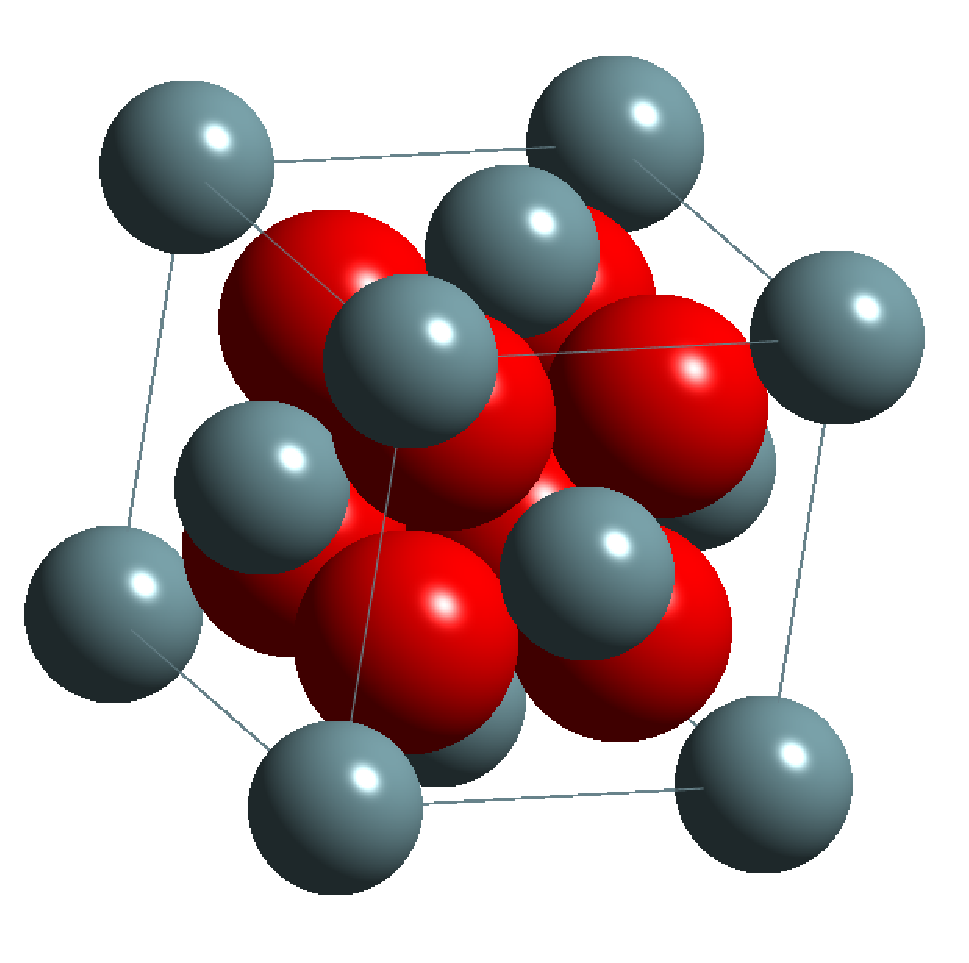
\includegraphics[scale=0.7]{Images/UO2}
\vspace{-10pt}
\caption[Example of the fluorite crystal structure.]{\label{fig:uo2Lattice}An image representing the fluorite crystal structure.  For UO\textsubscript{2}, the smaller spheres indicate the uranium atoms, and the larger spheres indicate the oxygen atoms.  Image courtesy of the University of Cambridge under the Creative Commons license.}
\vspace{-10pt}
%\end{figure}
\end{wrapfigure}
Today's nuclear reactors primarily use uranium dioxide (UO\textsubscript{2}) as their fuel source.\cite{uraniumInfo}  Understanding the properties of UO\textsubscript{2} requires an analysis of the basic crystal structure of the material.  The ceramic material UO\textsubscript{2} has a series of crystal lattices joined together in various ways (called twist, tilt, or mixed boundaries) to create it.  This material has a fluorite crystal structure, where the uranium atoms form a face-centered cubic (fcc) lattice, and the oxygen atoms form a simple cubic lattice within the fcc frame (see \Cref{fig:uo2Lattice}).

Understanding the various properties of the fuel allows nuclear reactors to run as safely and effectively as possible.  A few of these properties include thermal conductivity (how well heat flows through the material), fission gas release (how some of the fission products move throughout the material as gases), and mechanical stability (i.e. how the material bends or cracks under pressure or heat).  Taking thermal conductivity as an example, knowledge of this material property allows the most effective use of coolant to keep the reactor within operating temperatures, maximizing both efficiency and safety.  Knowledge of other material properties allows for similar gains in efficiency, safety, or both.

Interest in understanding UO\textsubscript{2} while in-reactor has led to efforts to more deeply understand the properties of the material.  Currently, Idaho National Laboratory (INL) faces the challenge of not having a completely accurate model of grain boundary energy anisotropy.  The current model assumes an isotropic energy, and this leads to an inability to model the material parameters correctly while in-reactor.  This in turn makes efforts in nuclear energy less efficient and/or safe than it otherwise could be.  INL aims to accurately model nuclear fuel while in-reactor, allowing accurate predictions regarding how the material properties will change.

This work adds to the safety and efficiency of using nuclear energy by providing the necessary information to accurately calculate the material properties of UO\textsubscript{2} in-reactor.  Specifically, this work improves the fitting parameters for grain boundary (GB) energy interpolation for UO\textsubscript{2} by using molecular dynamics (MD) results calculated by Zhang\cite{zhang2016} and Hansen\cite{hansen2016} with an anneal of 800 K.  Furthermore, this work begins preliminary efforts towards using more accurate functions to describe GB energy behavior.  Previous data did not use annealed crystal structures\cite{harbison2015}, which prevented the atoms from finding their ideal energetic minimum.  The 800 K anneal allows the atoms to relax to a value closer to their global minimum, as shown in \Cref{results}.  A database will store these simulated energies, and a MATLAB\textsuperscript{\textregistered} script will use the database to fit the function parameters.  INL will incorporate the updated parameters into its mesoscale phase field modeling platform MARMOT for use in modeling nuclear fuels.  As the modeling software incorporates these parameters, various tests of the UO\textsubscript{2} fuel can determine how the material properties change while in-reactor.

\chapter{Background\label{background}}
Tiny crystals called \emph{grains} make up every polycrystalline materials (such as ceramics).  The orientation of each grain does not generally depend on the orientation of the surrounding grains. Therefore, depending on how the crystal formed,\cite{callister2003} the crystal structures will possibly not line up at the interfaces where two grains meet.  This ``atomic mismatch"\cite{callister2003} leads to broken or stretched atomic bonds where atoms will not line up relative to a perfect crystal structure, creating defects called grain boundaries (GBs, see \Cref{fig:gb}). The most popular way to parameterize a GB uses the five degree-of-freedom (DoF) model.\cite{patala2013, lejcek2010, homer2015, bulatov2014, harbison2015, rohrer2011}.  This model only uses the macroscopic DoFs (the observable DoFs corresponding to the misorientation and inclination), ignoring the three translational DoFs (the ability of the grain to move or slide anywhere in space) possessed by each grain.  Three of the five DoFs specify the misorientation (or misalignment) of the grains with respect to each other.  The other two DoFs specify the orientation of the grain boundary plane (called the inclination).  The rotation axis and angle define the misorientation DoFs, and the GB normal defines the inclination DoFs.\cite{lejcek2010}

Three specific types of GBs occur in polycrystalline materials: twist, tilt, and mixed GBs.\cite{lejcek2010, rohrer2011}  These GBs describe the misorientation of two grains with respect to each other.  Twist boundaries have the axis of rotation between the two grains and the GB normal parallel to each other. Tilt boundaries can be either symmetric or asymmetric.  A perpendicular relationship between the axis of rotation and the GB normal creates a tilt boundary.  Symmetric tilt GBs have a boundary plane as a mirror plane: the atoms on one side of the boundary plane mirror the other side.  This makes the angles between the boundary plane and the orientation axes of the two grains equal. Asymmetric tilt boundaries have unequal angles.  \Cref{fig:misorientation} shows a representation of tilt boundaries (top) and twist boundaries (bottom).  A mixed GB combines twist and tilt boundary characteristics.

\begin{figure}[ht!]
\vspace{-20pt}
 \centering
 
 \subfloat[]{\label{fig:gb}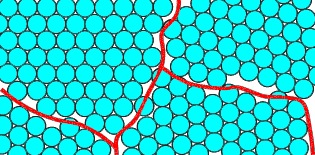
\includegraphics[scale=.9]{Images/grainBoundary}}\quad
 \subfloat[]{\label{fig:misorientation}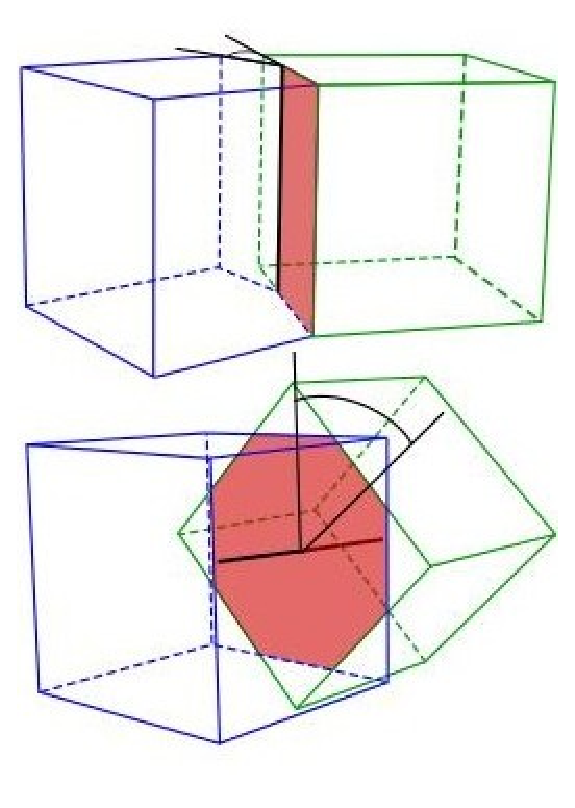
\includegraphics[scale=.6]{Images/twistTilt}}\quad
 \caption[Examples and types of grain boundaries.]{\label{gbs} A representation of GBs, where \protect\subref{fig:gb} shows an example of a grain boundary and \protect\subref{fig:misorientation} shows an example of GB types.  In \protect\subref{fig:gb} circles represent individual atoms of the grains, and the line represents the grain boundary.  Atomic mismatch between the differently oriented grains causes an excess of energy within the material, which has an effect on the material's properties.  Image courtesy of the University of Cambridge under the Creative Commons license. In \protect\subref{fig:misorientation} the tilt GB (top) has a perpendicular relationship between the axis of rotation and the GB normal, while the twist GB (bottom) has a parallel relationship between the two.  Image courtesy of Wikipedia under the Creative Commons license.}
\end{figure}

GBs have various effects on material properties, making them important to understand.\cite{patala2013, homer2015, bulatov2014}  The crystal structure has extra energy because of the atomic mismatch at the boundaries.  This extra energy, called GB energy, gives rise to GB motion.  Knowing and predicting how the GBs will move allows for more accurate calculations of a material's properties.  Thus, GB energy needs to be understood to accurately model the evolution of material properties.

Two methods, isotropic and anisotropic, model GB energy (among others).  The isotropic model most commonly (and most easily) describes GB energy.  This model ignores the impact of inclination on the GB energy, and assumes equal inclinations for a given misorientation, reducing the five-dimensional (5D) parameter space to a three-dimensional (3D) parameter space.  Historically, isotropic models assumed that the inclination had little or no impact on the GB energy.  Later, researchers used this model because of the difficulty in creating a full five DoF model.\cite{homer2015}  Alternatively, the anisotropic approach seeks to quantify the effect that misorientation \emph{and} inclination have on the GB energy.  Currently, researchers acknowledge the need for a full five DoF model of GB energy, but assert the difficulty inherent in developing such a model.\cite{rohrer2011, lejcek2010, homer2015}  Despite these difficulties, GB energy functions for certain materials, namely fcc metals copper, gold, aluminum, and nickel, have proven successful.\cite{bulatov2014} Recently,\cite{harbison2015} similar efforts created a GB energy function for UO\textsubscript{2}.  This work improves the accuracy of that energy interpolation function.

\chapter{Methods\label{methods}}
Any fitting procedure requires a sufficient amount of data, but unfortunately such data does not exist for uranium dioxide (UO\textsubscript{2}) in the literature.  As a work-around, this work used molecular dynamics (MD) simulations\cite{zhang2016,hansen2016} as fitting data to calculate the GB energies of various lattices based on the coincident site lattice (CSL) model. This model builds off of the idea that the GB energy has lower values when more lattice sites coincide.  A number defined as the $\Sigma$-number describes the number of coincident sites per total number of lattice sites in a given unit cell of a crystal.\cite{lejcek2010, rohrer2011} This work developed a MATLAB\textsuperscript{\textregistered} script using Bulatov \emph{et al.}'s methods\cite{bulatov2014} and building off of Harbison's script\cite{harbison2015} to fit parameters to the gathered data.  A reduced chi-square statistic determined the effectiveness of the fit.

\section{Molecular Dynamics\label{methods:MD}}
Zhang\cite{zhang2016} and Hansen\cite{hansen2016} collected simulation results from the Large-scale Atomic/Molecular Massively Parallel Simulation (LAMMPS) software (developed at Sandia National Laboratory\cite{plimpton1995}) for a number of twist, tilt, and mixed GBs.  They performed these calculations by simulating two crystals of UO\textsubscript{2} and placing them together in various orientations.  A GB forms at the interface, creating GB energy.  Calculating the energy of the system from the interatomic forces inside the crystal, and comparing that energy to the energy of a single grain (of the same size as the combined two grains) determines the energy at the GB.\cite{harbison2015}  Calculating the GB energy follows the form:\cite{butterfield2013}
\begin{equation}\label{eq:GBE}
E_{\textnormal{GB}}=\frac{|E_{\textnormal{single grain}} - E_{\textnormal{two grains}}|}{2A_{\textnormal{GB}}}.
\end{equation} 
Here, $E_{\textnormal{GB}}$ represents the energy at the grain boundary, and $E_{\textnormal{single grain}}$ and $E_{\textnormal{two grains}}$ represent the energies of the single and double grains respectively.  $A_{\textnormal{GB}}$ represents the area of the grain boundary.  \Cref{fig:lammps} shows an example of how the atoms align. Harbison's original calculations\cite{harbison2015} used no anneal ($T_{\textnormal{max}}\approx0$ K), only allowing the atoms to relax to their local minima.  This work used an anneal of 800 K, allowing the atoms to relax to a better estimate of their global minimum value as shown in \Cref{results}.  This work used the same misorientation angles for the GB energy calculations that Harbison used.  The fitting procedure uses these energies to produce parameters describing the five-dimensional GB space.

\begin{figure}[ht!]
 \centering
 
 \subfloat[]{\label{fig:lammps1}\includegraphics[scale=0.287]{"Images/LAMMPS example image"}}\quad
 \subfloat[]{\label{fig:lammps2}\includegraphics[scale=0.3]{"Images/LAMMPS example image2"}}\quad
 \caption[An example of crystal structure after annealing.]{\label{fig:lammps}These figures demonstrate example crystal structures of UO\textsubscript{2} after an annealing process.  The better the atoms line up, the lower the energy. \protect\subref{fig:lammps1} shows an example of a mostly aligned GB, indicative of a lower energy.  \protect\subref{fig:lammps2} shows an example of a misaligned GB, indicative of a higher energy.  These two images show results from a \textlangle{}111\textrangle{} twist simulation.  Different viewpoints show different amounts of alignment.  The LAMMPS simulation package takes care of all the calculations to determine the energy at these GBs. Images courtesy of Dr. Evan Hansen, used with permission.}
\end{figure}

\section{Bulatov \emph{et al.}'s Methods\label{methods:bulatov}}
This work implemented Bulatov \emph{et al.}'s hierarchical interpolation method to find the energy of an arbitrary GB in the five-space.\cite{bulatov2014}  They chose three three-dimensional (3D) axes with at least two-fold symmetry (called high-symmetry axes) to use as scaffolding to build the entire five-dimensional (5D) function.  Bulatov \emph{et al.}\ and this work chose the \textlangle{}100\textrangle{}, \textlangle{}110\textrangle{}, and the \textlangle{}111\textrangle{} sets for their four-, two-, and three-fold rotational symmetries respectively.\footnote{Symmetry operations for cubic crystals include rotating by 90\textdegree{}, 180\textdegree{}, or 120\textdegree{} about any \textlangle{}100\textrangle{}, \textlangle{}110\textrangle{}, or \textlangle{}111\textrangle{} axis respectively.\cite{stokes2007}  Thus, the \textlangle{}100\textrangle{} set has four-fold symmetry (360\textdegree{}$/90$\textdegree{}$=4$), the \textlangle{}110\textrangle{} set has two-fold symmetry (360\textdegree{}$/180$\textdegree{}$=2$), and the \textlangle{}111\textrangle{} set has three-fold symmetry (360\textdegree{}$/120$\textdegree{}$=3$).}  Each 3D subset builds from interpolation of its own one- and two-dimensional subsets.  The symmetric tilt and twist GBs for each set were fitted first because of their simplicity.  The rotation angle fully defines the energies for these subsets, making them one-dimensional (in \Cref{fig:bulatov5D}, the darker bands in the smaller circles).  Having the parameters from the symmetric tilt subset allows interpolation to the asymmetric, or general, tilt subset.  A second rotation angle defining the rotation of the second grain makes this subset two-dimensional (the lighter, wider band around the symmetric subset).  A combination of the general tilt (two dimensions) and the twist subsets (one dimension) interpolates the 3D subset for each high-symmetry axis (the three smaller circles).  Bulatov \emph{et al.}\ and this work used these three 3D subsets to interpolate the GB 5D space. \Cref{fig:bulatovRodrigues} shows the simplified GB space using the Rodrigues fundamental zone representation. \Cref{app:gbRep} provides a further explanation of Rodrigues space and the fundamental zone.

Bulatov \emph{et al.}\ and this work used the Read-Shockley-Wolf (RSW) functions,\cite{wolf1989} which take the form:
\begin{equation}
E_{min} + (E_{max} - E_{min})\ \textnormal{sin}\left(\frac{\pi}{2}\frac{\theta-\theta_{min}}{\theta_{max} - \theta_{min}}\right)\left(1-a\textnormal{log}\left(\textnormal{sin}\left(\frac{\pi}{2}\frac{\theta-\theta_{min}}{\theta_{max} - \theta_{min}}\right)\right)\right),
\end{equation}
where $\theta$ is the misorientation angle, $\theta_{min}$ and $\theta_{max}$ represent the minimum and maximum angles on the domain respectively, $a$ is a shaping parameter, and $E_{min}$ and $E_{max}$ represent the energy at $\theta_{min}$ and $\theta_{max}$ respectively.  Each RSW function covers a ``low-angle" subset (around 15\textdegree{}, with larger domains being less accurate)\cite{rohrer2011,wolf1989} of the domain in the 1D GB space.  \Cref{fig:RSW} shows an example of a simple RSW function.  Stitching together multiple RSW functions forms the 1D subsets.

\begin{figure}[ht!]
 \centering
 \subfloat[]{\label{fig:bulatov5D}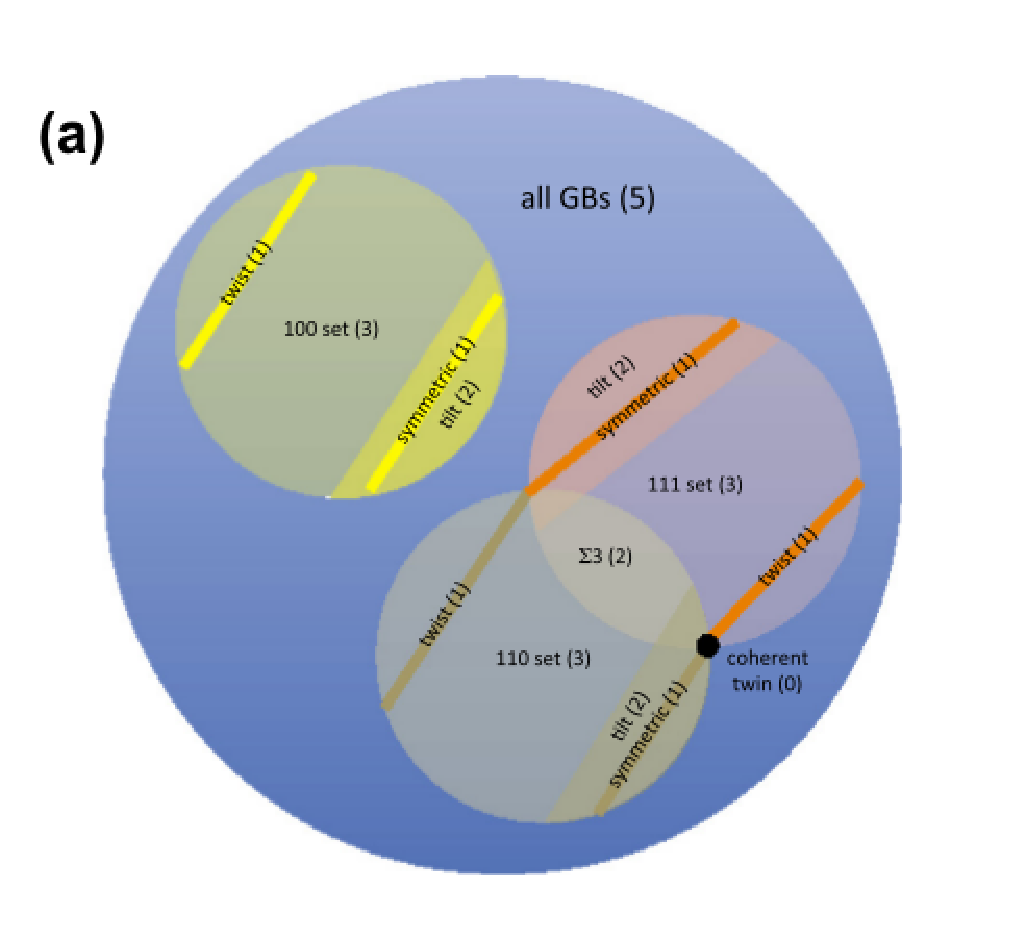
\includegraphics[scale=0.42]{Images/bulatov_5D_model}}\quad
 \subfloat[]{\label{fig:bulatovRodrigues}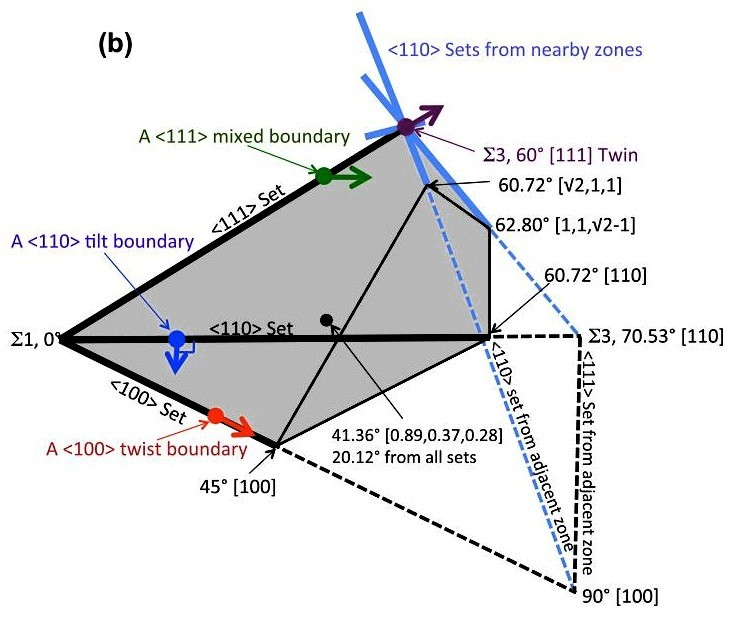
\includegraphics[scale=0.32]{Images/bulatov_rodrigues}}
 \caption[The theoretical relationship between high-symmetry subsets and fundamental zone.]{\label{fig:bulatovFig2}Figure 2 from Bulatov \emph{et al.}\cite{bulatov2014} \protect\subref{fig:bulatov5D} demonstrates the theoretical relationship between the high-symmetry subsets of the 5D GB space.  Each multi-dimensional subset interpolates from smaller-dimensional subsets. \protect\subref{fig:bulatovRodrigues} shows the Rodrigues space representation of the fundamental zone of all GBs as built from three high-symmetry axes (\textlangle{}100\textrangle{}, \textlangle{}110\textrangle{}, and \textlangle{}111\textrangle{}).  The unit vectors along the axis identify the boundary plane inclination in the frame of grain one.  A parallel vector thus represents a twist boundary, a perpendicular vector represents a tilt boundary, and neither parallel nor perpendicular vectors represent a mixed boundary.}
\end{figure}

\begin{figure}[ht!]
 \centering
 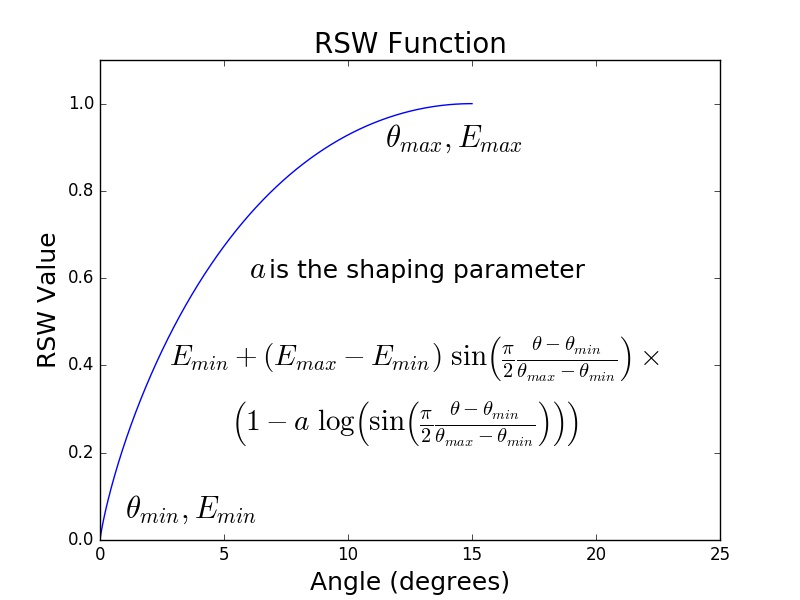
\includegraphics[scale=0.5]{Images/rsw}
 \caption[The general form of an RSW function.]{\label{fig:RSW}An example of an RSW function with $\theta_{min} = 0$\textdegree{}, $\theta_{max} = 15$\textdegree{}, and $a$ (the shaping parameter) $= 0.5$.  Combining these functions into a Piecewise set over a given domain gives the GB energy curves their distinct, cusp-like behavior.  The RSW functions scale based on $E_{min}$ and $E_{max}$.  In this example, $E_{min} = 0$ and $E_{max} = 1$. Note that $E_{min}$ and $E_{max}$ do not represent the lowest and highest energies in the domain, but rather represent the energy at $\theta_{min}$ and $\theta_{max}$ respectively, meaning that the value of $E_{min}$ could be higher than the value of $E_{max}$.}
 % NOTE!!! using \degree WILL NOT WORK!
\end{figure}



\section{Code Analysis\label{methods:code}}
Harbison\cite{harbison2015} and Bulatov \emph{et al.}\cite{bulatov2014}\ developed MATLAB\textsuperscript{\textregistered} scripts for their work.  This work analyzed these codes and used the ideas from them to develop the code that generated the parameters listed in \Cref{app:params}.

\subsection{The Fitting Code\label{code:fitting}}
This work performed an extensive analysis of Harbison's code to learn how it works and to implement the ideas therein.  The basic outline for the fitting procedure follows.  First, a database containing energies associated with either a twist or tilt GB on one of the three high-symmetry axes provides the fitting data.  A separate database provides the test parameters which define starting points for the fitted parameters.  The parameters found from the 1D fits assist in fitting the higher-dimensional sets.  Important angles specify where to expect low energies, such as the $\Sigma5$ boundary for the \textlangle{}100\textrangle{} symmetric tilt subset.  The $\Sigma$-number from CSL theory determines the angles. Because the $\Sigma$-number designates the number of lattice points between each coincident site (and assuming the separation distance between each lattice site, or the lattice constant is known) the angle of the GB misorientation can be determined.  A value known as the $e_{RGB}$ parameter scales every energy in the parameter vector to minimize the potential for error in calculations. The $e_{RGB}$ parameter represents the energy of an arbitrary, random GB, and represents an average of the material's GB energies.  Thus, making relevant comparisons requires unscaling the energies based on the units of energy desired (typically J/m\textsuperscript{2}).  All of the parameters and the angle-energy pairs from the database get passed into a grid-search fitting function.  This work gave each subset a different initial step size to avoid a numerical error where the steps would take the angles currently being looked at outside of their domain. Without this, the grid-search procedure would not return the correct amount of values, preventing the code from running to completion.

After fitting the six one-dimensional subsets and the three two-dimensional subsets, interpolating the twist (1D) and asymmetric tilt (2D) subsets calculates the mixing parameters to fit the three-dimensional subsets.  The mixing parameters define the relationship between the twist and general tilt subsets within a high-symmetry axis - i.e. the relationship between the small dark bands representing the twist boundaries and the lighter, wider bands representing the tilt boundaries in \Cref{fig:bulatov5D}.  The final step calculates the weighting parameters, which defines the relationship between the three high-symmetry subsets.  Equations defining the various relationships can be found in Bulatov \emph{et al.}'s work.\cite{bulatov2014}

\subsection{The Energy Calculation Code\label{code:energyCalc}}
Bulatov \emph{et al.}'s open-source MATLAB\textsuperscript{\textregistered} code\cite{bulatov2014}, \lstinline!GB5DOF.m!, calculates the energy of an arbitrary GB in certain fcc metals. This work uses this script for calculating an arbitrary GB in UO\textsubscript{2}, and proceeds as follows.  First, it compares all symmetrically equivalent representations of a GB (on a per-axis basis) to calculate metrics defining the ``distance" between the GB and all three high-symmetry axes (for cubic crystals, there are 24 equivalent representations\cite{stokes2007}).  Because of the three, six, and four unique axes for the \textlangle{}100\textrangle{}, \textlangle{}110\textrangle{}, and \textlangle{}111\textrangle{} sets respectively, the script calculates a maximum of $6\times24=144$ distances, afterwards discarding any that exceed a predefined cutoff distance.  After calculating all distances, the script keeps only the unique representations to avoid double-counting.\cite{bulatov2014}  It then calculates energies for each unique distance in each subset, then weights and sums them to give the interpolated energy for the specified GB.

\section{Reduced Chi-Square Statistic\label{methods:chi2}}
A good way to test how well a function fits the data uses a reduced chi-square goodness-of-fit statistic.\cite{bevington2003}  Bulatov \emph{et al.}'s function required the orientation matrices (which Bulatov \emph{et al.}\ calls the P and Q matrices for the first and second grains respectively) as input parameters to calculate this statistic.  These three by three matrices specify the orientation in a lab frame of the two grains individually. A good fit will have a reduced chi-square value close to one, while those values greater than one indicate an under fit, and those values less than one indicate an over fit.\cite{bevington2003}

\subsection{Developing the P and Q Matrices\label{chi2:PQ}}
This work created the P and Q matrices.  Because of the vast quantity of work done with crystallography over the past few decades, many different methods can specify the orientation matrices of grains. A rotation matrix also needed to be calculated which rotates the axis of rotation to the [100] direction, as Bulatov \emph{et al.}'s energy calculation code assumes.  This work used three methods, following the method prescribed in MARMOT, using the Rodrigues rotation formula, and using the Bunge rotation matrix, in the process of developing these matrices.

\subsubsection{MARMOT Method\label{PQ:MARMOT}}
MARMOT, Idaho National Laboratory's (INL's) mesoscale phase-field modeling platform,\cite{tonks2012} calculates the P and Q matrices for the grains using Euler angles as input parameters.  MARMOT uses the Bunge convention to convert the Euler angles to orientation matrices.  The Bunge convention uses the $ZXZ$ or $ZX'Z''$ rotation set, which rotates first about the \emph{z} axis, then the rotated \emph{x} axis, and finally about the rotated \emph{z} axis.  Multiplying the \emph{z}, \emph{x} and \emph{z} rotation matrices together in that order generates the formula to convert from Bunge Euler angles to the rotation matrix:

\begin{equation}
\label{eq:bungeMat}
\left[
\begin{array}{ccc}
c_1\ c_3 - c_2\ s_1\ s_3 & -c_1\ s_3 - c_2\ c_3\ s_1 & \phantom{-}s_1\ s_2 \\
c_3\ s_1 + c_1\ c_2\ s_3 & \phantom{-}c_1\ c_2\ c_3 - s_1\ s_3 & -c_1\ s_2 \\
s_2\ s_3 & \phantom{-}c_3\ s_2 & \phantom{-}c_2 
\end{array}
\right]
\end{equation}
where $c_\textnormal{n}$ and $s_\textnormal{n}$ represent the cosine and sine of the respective angles (1 represents the first \emph{z} rotation, 2 represents the \emph{x} rotation, and 3 represents the second \emph{z} rotation, usually referred to as\cite{randle2000} $\varphi_1$, $\Phi$, $\varphi_2$).

MARMOT calculates the rotation matrix using the GB normal by finding the rotation matrix required to rotate that vector to the [100] direction.  In MARMOT, input files set up the simulations.  In the input files different sections (called blocks) specify material parameters, boundary conditions, initial conditions, and the physical models to use to solve the problem (among others).  A horizontal or vertical boundary for tilt or twist GBs respectively defined the initial condition used to calculate the rotation matrices in MARMOT for this set of problems.  Because of this set up, tilt boundaries had GB normals along the [010] axis, and twist boundaries had GB normals along the [$\bar{1}$00] axis.

\subsubsection{Rodrigues Rotation Formula\label{PQ:RRF}}
The Rodrigues rotation formula\cite{belongie2006} (RRF) calculates the rotation matrices given an axis and an angle using the following formula:
\begin{equation}
\label{eq:rrf}
\bm{R} = \bm{I} + \textnormal{sin}\ \theta\ \bm{K} + (1 - \textnormal{cos}\ \theta)\ \bm{K}^2,
\end{equation}
where $\bm{I}$ is the 3x3 identity matrix, $\theta$ is the angle rotated through, and $\bm{K}$ is the skew-symmetric matrix formed by the axis of rotation ($\bm{a}$, where $\bm{a}$ has components $a_x$, $a_y$, and $a_z$) by:
\begin{equation}
\label{eq:skewSymMat}
\left[
\begin{array}{ccc}
\phantom{-}0 & -a_z & \phantom{-}a_y \\
\phantom{-}a_z & \phantom{-}0 & -a_x \\
-a_y & \phantom{-}a_x & \phantom{-}0
\end{array}
\right].
\end{equation}

This work calculated the rotation matrices two different ways with this orientation matrix formulation.  The first method used the MARMOT-generated rotation matrices.  A second method calculated the rotation matrices using geometric arguments (see \Cref{fig:PlaneNorms}).  From the geometric arguments this work identified the normals given in \Cref{table:geometricgbnorms}.  \Cref{app:RotationMatrix} shows the code used to generate the rotation matrices.

\begin{figure}[ht!]
\begin{minipage}{0.33\linewidth}
 \centering
 \subfloat[]{\label{fig:100TwistPlane}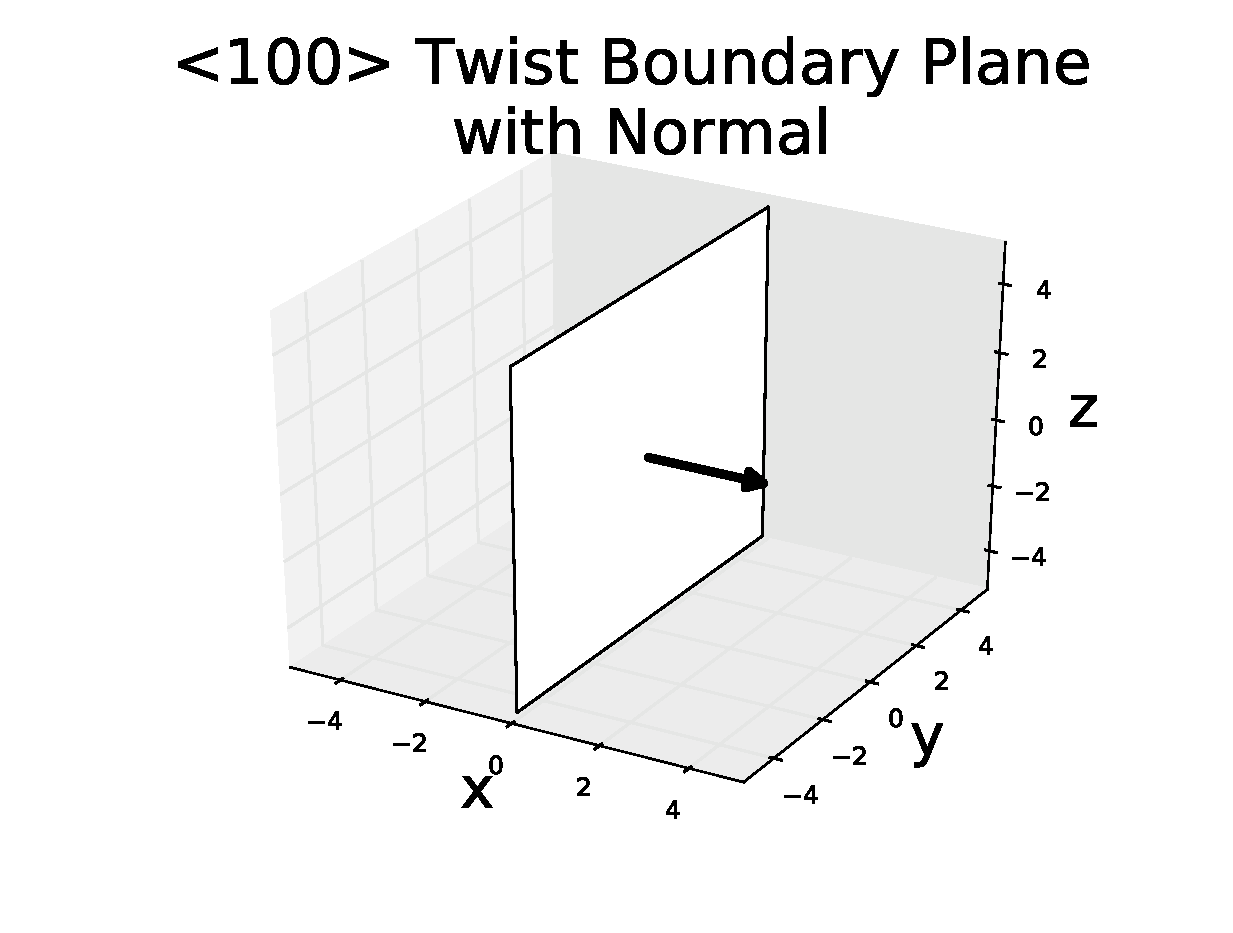
\includegraphics[scale=0.2]{Images/Twist100Plane}}
\end{minipage}%
\begin{minipage}{0.33\linewidth}
 \centering
 \subfloat[]{\label{fig:110TwistPlane}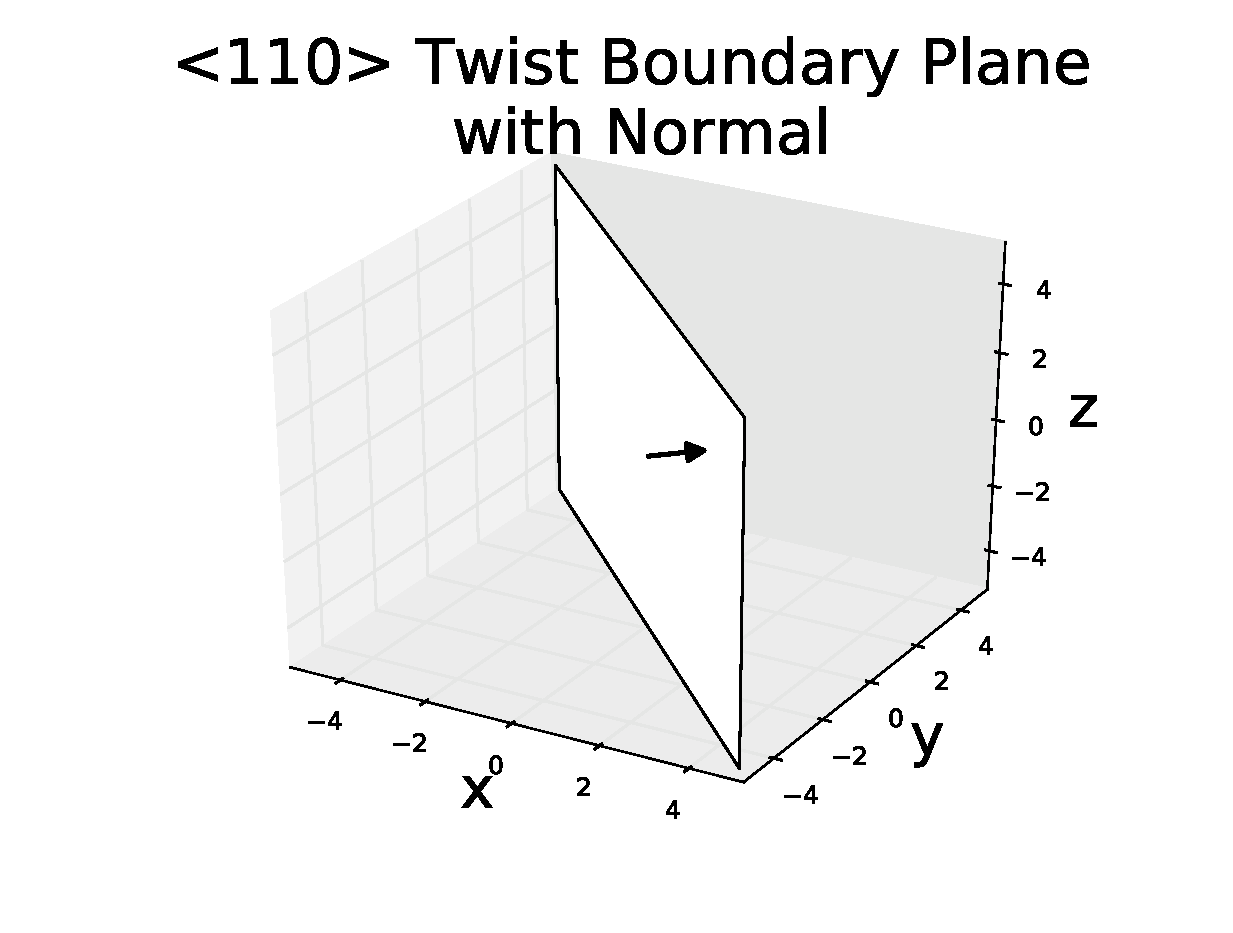
\includegraphics[scale=0.2]{Images/Twist110Plane}}
\end{minipage}%
\begin{minipage}{0.33\linewidth}
 \centering
 \subfloat[]{\label{fig:111TwistPlane}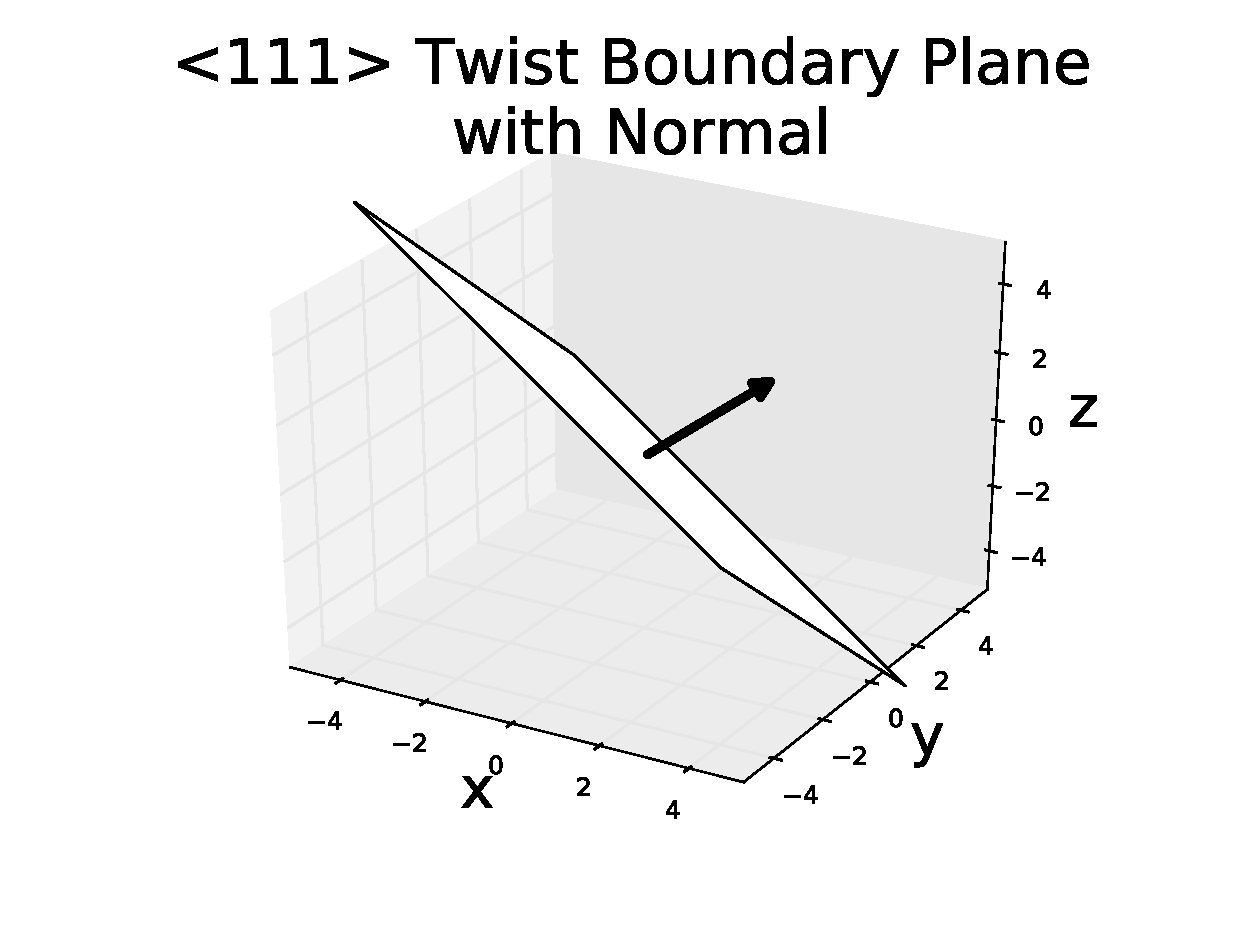
\includegraphics[scale=0.2]{Images/Twist111Plane}}
\end{minipage}
 \centering
 
 \subfloat[]{\label{fig:100TiltPlane}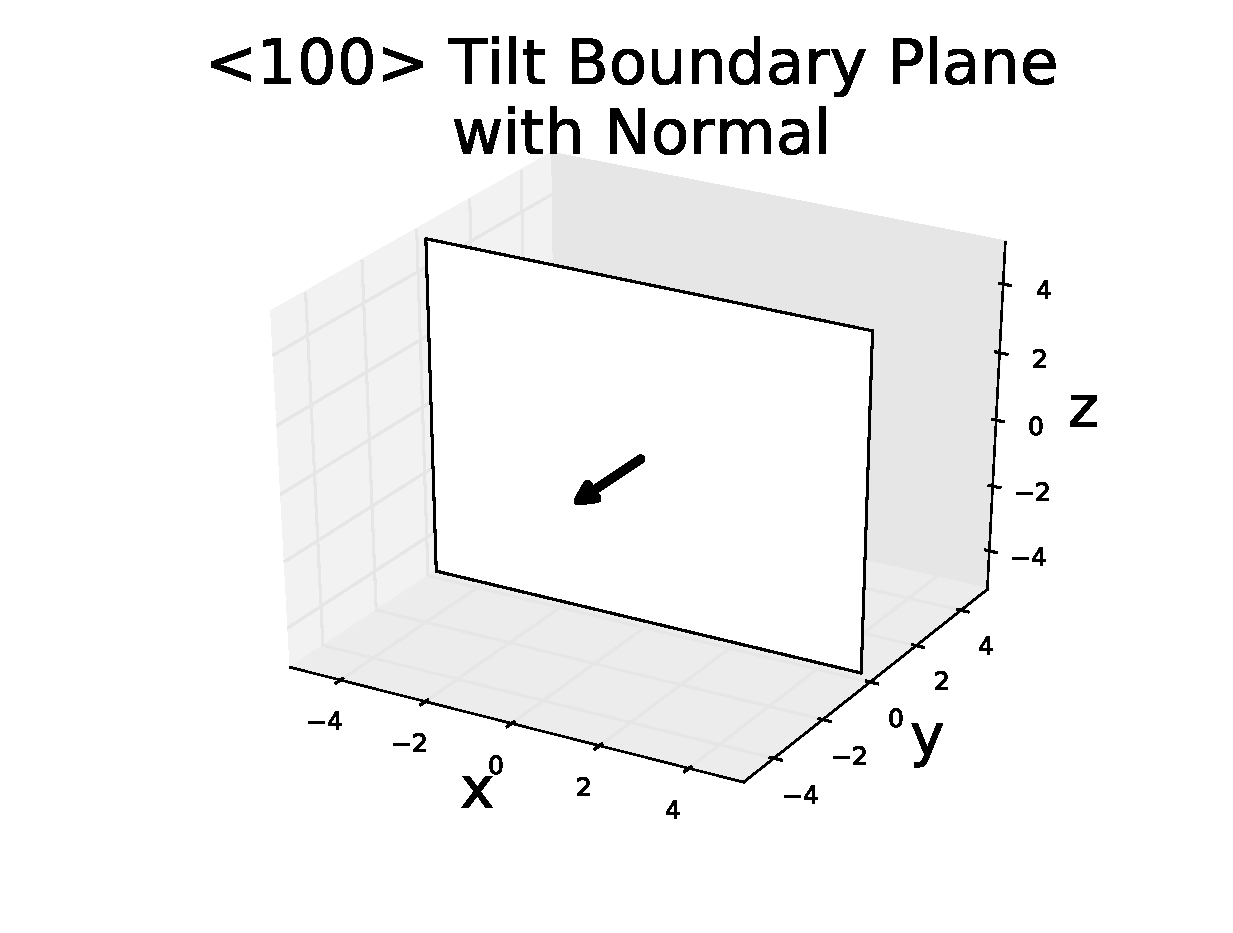
\includegraphics[scale=0.2]{Images/Tilt100Plane}}\quad
 \subfloat[]{\label{fig:110TiltPlane}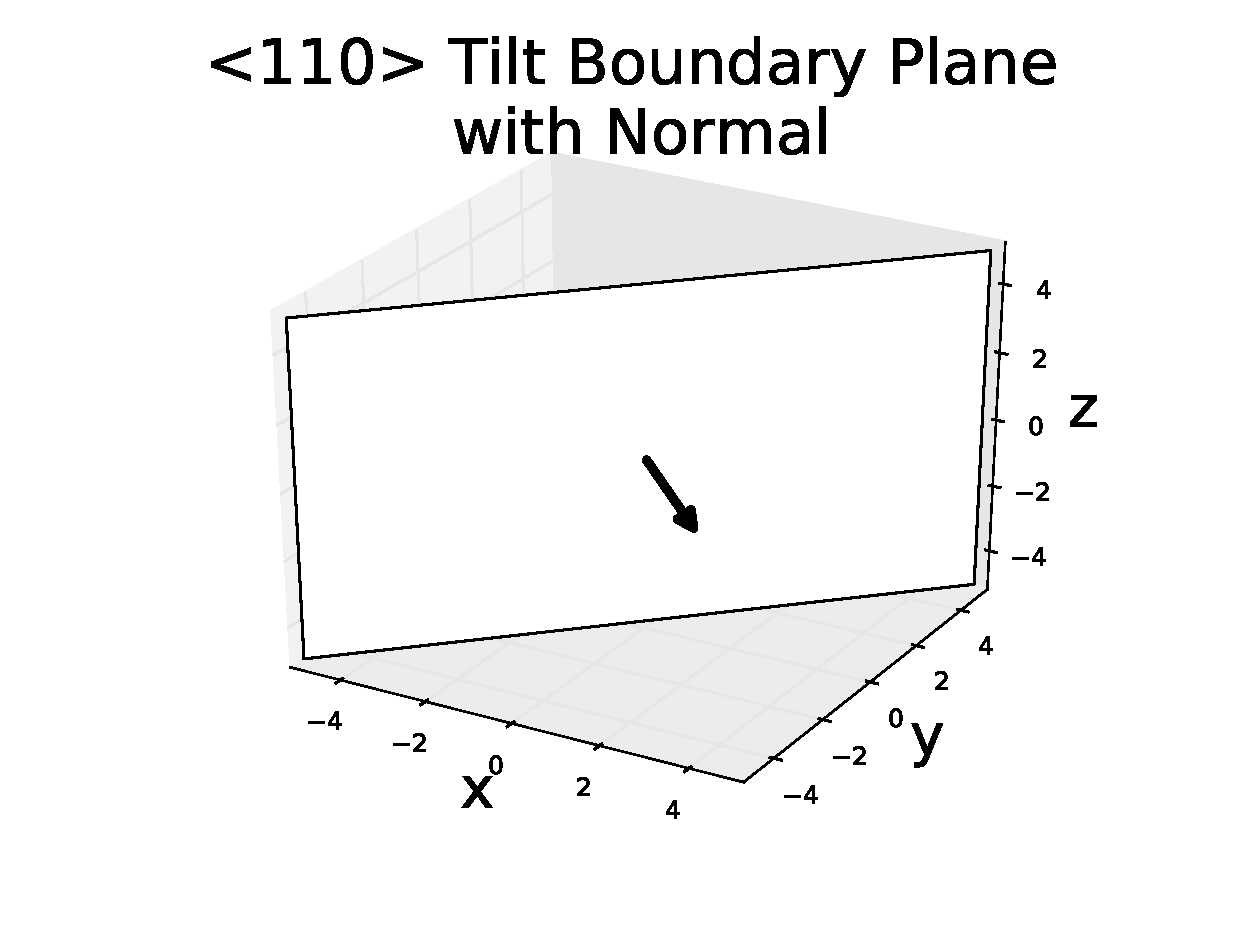
\includegraphics[scale=0.2]{Images/Tilt110Plane}}\quad
 \caption[Geometric method of determining grain boundary normals.]{\label{fig:PlaneNorms}A geometric method of determining the normals of a GB.  \protect\subref{fig:100TwistPlane} to \protect\subref{fig:111TwistPlane} show the normals for a GB perpendicular to the axis of rotation (a twist GB).  The axis about which the grains rotate defines the GB normal. \protect\subref{fig:100TiltPlane} and \protect\subref{fig:110TiltPlane} show the normals for a GB parallel to the axis of rotation (a tilt GB).  The same GB normal for \textlangle{}110\textrangle{} tilt boundaries can be used for \textlangle{}111\textrangle{} tilt boundaries.}

\end{figure}

\begin{table}[ht!]
\centering
\caption{\label{table:geometricgbnorms}Table of GB normals for different GB types. The normalized dot product of the axis with the GB normal is zero in all tilt cases and one in all twist cases.  Each subset has two options for the grain boundary normals because of inversion symmetries.}

\begin{tabular}{ccc}
Axis & Boundary Type & GB Normal \\
\hline
\hline
\multirow{2}{*}{\textlangle{}100\textrangle{}} & \multirow{2}{*}{Tilt} & [010] \\
                              & & [0$\bar{1}$0] \\
\hline
\multirow{2}{*}{\textlangle{}110\textrangle{}} & \multirow{2}{*}{Tilt} & [1$\bar{1}$0] \\
							  & & [$\bar{1}$10] \\
\hline
\multirow{2}{*}{\textlangle{}111\textrangle{}} & \multirow{2}{*}{Tilt} & [1$\bar{1}$0] \\
							  & & [$\bar{1}$10] \\
\hline
\multirow{2}{*}{\textlangle{}100\textrangle{}} & \multirow{2}{*}{Twist} & [100] \\
							  & & [$\bar{1}$00] \\
\hline
\multirow{2}{*}{\textlangle{}110\textrangle{}} & \multirow{2}{*}{Twist} & [110] \\
							  & & [$\bar{1}\bar{1}$0] \\
\hline
\multirow{2}{*}{\textlangle{}111\textrangle{}} & \multirow{2}{*}{Twist} & [111] \\
							  & & [$\bar{1}\bar{1}\bar{1}$] \\
\hline
\hline
\end{tabular}
\end{table}

\subsubsection{Bunge Rotation Matrix\label{PQ:BungeMat}}
MARMOT uses the Bunge rotation matrix (see \Cref{eq:bungeMat}) to create the orientation matrices.  This work used various methods to calculate the Euler angles, of which three are briefly described here. The first two methods use the Euler angles to calculate the entirety of the rotation matrix.

First, this work tried to use scripts developed to calculate the various Euler angles for MARMOT.  These scripts did not work because of the same assumptions made earlier about the orientation of the GB, namely, that all pure tilt GBs have a normal of [010], and that all pure twist GBs have a normal of [$\bar{1}$00].  This work assumed boundary conditions to be either perpendicular or parallel to the rotation axis, while MARMOT's boundary conditions assume GB normals along the $x$- or $y$-axes.

The second method used an open-source MATLAB\textsuperscript{\textregistered} package called MTEX.\cite{bachmann2010}  This package calculates Euler angles using quaternions.  These Euler angles did not generate the correct results either, for the most part creating the same sorts of graphs as the MARMOT method.

The working method used the mathematics of quaternions directly.\cite{weisstein2004}  This work calculated the quaternions based on the misorientation axis and angle.  A quaternion is a four-dimensional vector containing one real part, and three imaginary parts, calculated as follows:
\begin{equation}
\label{eq:quat}
\bm{q}=\left[\textnormal{cos}\left(\frac{\theta}{2}\right),\ a_x\,\textnormal{sin}\left(\frac{\theta}{2}\right),\ a_y\,\textnormal{sin}\left(\frac{\theta}{2}\right),\ a_z\,\textnormal{sin}\left(\frac{\theta}{2}\right)\right],
\end{equation}
with axis $\bm{a}$ and misorientation angle $\theta$.  After converting the axis and misorientation angle to a quaternion, another conversion changes the quaternion to a set of Bunge Euler angles.  Calculation of the angles uses Python's \lstinline!atan2()! method, allowing all four quadrants in Cartesian space to be accounted for.
\begin{align}
\label{eq:quat2euler}
\begin{aligned}
\chi &= \sqrt{(q_0^2+q_3^2)(q_1^2+q_2^2)}\\
\varphi_1 &= \textnormal{atan2}\left(\frac{q_0q_2+q_1q_3}{2\chi}, \frac{q_0q_1-q_2q_3}{2\chi}\right)\\
\Phi &= \textnormal{atan2}\left(2\chi, q_0^2+q_3^2-q_1^2-q_2^2\right)\\
\varphi_2 &= \textnormal{atan2}\left(\frac{q_1q_3-q_0q_2}{2\chi}, \frac{q_0q_1+q_2q_3}{2\chi}\right).
\end{aligned}
\end{align}
Inputting the Euler angles into \Cref{eq:bungeMat} created the orientation matrices for the grains.  \Cref{app:OrientationMatrix,app:genOrientationMatrix} provide the codes used to generate the orientation matrices.

\subsubsection{Testing The Matrices\label{PQ:Testing}}
This work attempted to reproduce the 1D subset graphs as shown in Bulatov \emph{et al.}\ as a way to test the different methods.  Different methods experienced various levels of success.  \Cref{appfig:compare100,appfig:compare110,appfig:compare111} show the matrices giving the best results.

While the first method works well for MARMOT, the MATLAB\textsuperscript{\textregistered} script does not necessarily expect the same GB normal assumed by MARMOT.  Thus, the results coming from using this combination of matrices ended up working only for the \textlangle{}100\textrangle{} tilt, \textlangle{}110\textrangle{} tilt, and \textlangle{}100\textrangle{} twist subsets. The \textlangle{}110\textrangle{} twist subset had issues with singularities, and the \textlangle{}111\textrangle{} subsets did not remotely match the expected outcome.

\subsection{Calculating Reduced Chi Squared\label{chi2:chi2red}}
This work used two methods to calculate the $\chi^2_{\textnormal{red}}$ statistic.  The first method used the P and Q matrices as developed above to test the entirety of the fit.  The second method calculated the statistic for each 1D subset, then calculated the full $\chi^2_{\textnormal{red}}$ value using the statistics from the subsets.  \Cref{results} discusses the results from these calculations.

The test for the entire fit used the P and Q matrices to calculate the energy in 1\textdegree{} intervals for each subset, using Bulatov \emph{et al.}'s \lstinline!GB5DOF.m! script.  This work used \Cref{eq:chi2} to calculate the $\chi_{\textnormal{red}}^2$ value for each subset and for the entire fit, producing the results in \Cref{table:chi2} under the 800 K anneal column under the ``$\chi_{\textnormal{red}}^2$ using P and Q matrices" section,

\begin{equation}
\label{eq:chi2}
\chi^2_{\textnormal{red}} = \frac{1}{N-n-1} \sum \frac{(\epsilon_{\textnormal{md}} - \epsilon)^2}{e\ \epsilon_{\textnormal{md}}}.
\end{equation}
In this equation, $N$ is the number of observations, $n$ is the number of parameters, $\epsilon_{\textnormal{md}}$ are the energies from MD, $\epsilon$ are the energies from the model, and $e$ is the uncertainty in the MD results.

Using the second method, the same angles used in the fitting procedure were used in the RSW equations that create the 1D subsets.  The differences between the values resulting from there and the MD simulation values lead to the $\chi_{\textnormal{red}}^2$ values shown in the 800 K anneal column under the ``$\chi_{\textnormal{red}}^2$ comparing the 1D fits" section.  This work implemented the same methods to calculate the $\chi_{\textnormal{red}}^2$ values for the data without an anneal.

The statistic calculated using these methods differs from the $\chi^2$ statistic used in the grid-search function to calculate the fitting parameters.  The grid-search function used \Cref{eq:chi2grid}, and generated values of the same order as \Cref{eq:chi2}.

\begin{equation}
\label{eq:chi2grid}
\chi^2=\sum (E_{\textnormal{measured}} - E_{\textnormal{calculated}})^2
\end{equation}

\chapter{Results and Discussion\label{results}}
\section{Validation of P and Q Matrices\label{results:PQValid}}
Comparison of the energy profiles calculated from the P and Q matrices with the copper energy profiles expected from the parameters defined in Bulatov \emph{et al.}'s code provides a way to validate the generated matrices.  \Cref{fig:compare100} shows the results from this comparison for the \textlangle{}100\textrangle{} set, with all six subsets shown in \Cref{appfig:compare100,appfig:compare110,appfig:compare111}.  The calculated energies match exactly the predicted values for all but a few points.  Each data set does not match the expected energy at 1\textdegree{}, and the tilt data sets also see this mismatch at their second to last data point.

\begin{figure}[ht!]
 \centering
 
 \subfloat[]{\label{fig:compare100Twist}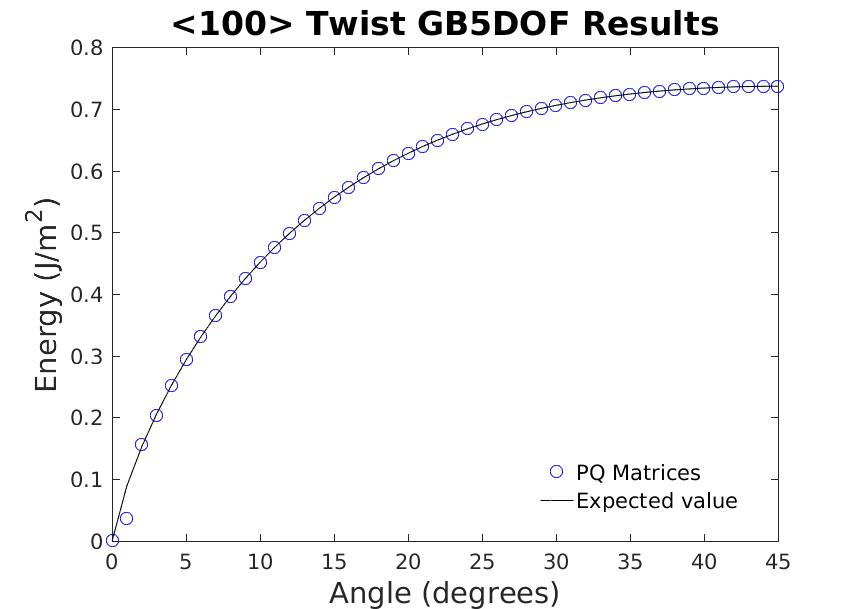
\includegraphics[scale=0.24]{Images/TestPQFit100Twist}}\quad
 \subfloat[]{\label{fig:compare100Tilt}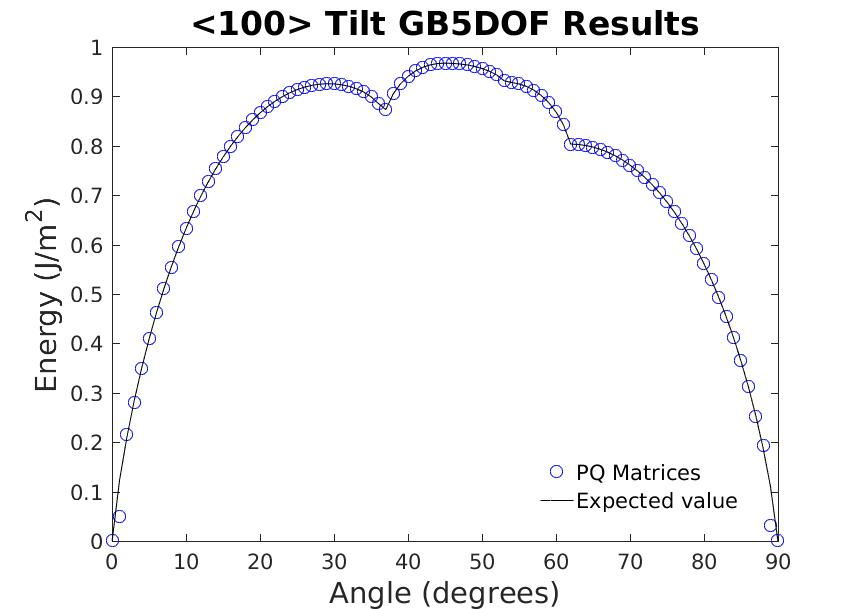
\includegraphics[scale=0.26]{Images/TestPQFit100Tilt}}
 \caption[A comparison of the \textlangle{}100\textrangle{} copper curve with the calculated results.]{\label{fig:compare100} The \textlangle{}100\textrangle{} twist \protect\subref{fig:compare100Twist} and tilt \protect\subref{fig:compare100Tilt} results for the P and Q matrices as compared to Bulatov \emph{et al.}'s energy profiles. Bulatov \emph{et al.}'s \lstinline!GB5DOF.m! MATLAB\textsuperscript{\textregistered} script calculated the expected values by using the default parameters.  The \lstinline!GB5DOF.m! script calculated the values using the generated matrices. With the exception of the data points at 1\textdegree{} in both \protect\subref{fig:compare100Twist} and \protect\subref{fig:compare100Tilt} and 89\textdegree{} in \protect\subref{fig:compare100Tilt}, the energies calculated from the matrices matches the expected curves exactly.}
\end{figure}

\section{Fitting Results\label{results:fit}}
\Cref{fig:100,fig:110,fig:111} compare the one-dimensional (1D) results from Harbison\cite{harbison2015} and this work.  The results show a general decrease in the grain boundary (GB) energies, allowing trends in the different subsets to emerge.  These trends allow for an all around better fit, but also introduce some unexpected results.  \Cref{app:params} shows the parameters calculated from the fitting procedure.

Initial MD recalculations of the \textlangle{}100\textrangle{} symmetric tilt GB energies using the 800 K anneal (\Cref{fig:100Tilt}) showed an unexpected deep cusp around 28\textdegree{}.  An analysis of the molecular dynamics (MD) simulation results for this misorientation revealed that, in this case, abnormally high pressures had caused the two crystals to realign.  This realignment caused the misorientation angle to change, causing the GB energy to be much lower than expected.  Comparison with Harbison's simulation result revealed that the crystal structure from his simulation did not realign.  While Harbison's did not use annealed data and thus may not represent a global minimum, the data point follows the surrounding data's trend, justifying the use of his result.

Of the symmetric tilt GB energy sets, the \textlangle{}110\textrangle{} set has the most improvement.  All three sets showed a general decrease in the energy, increasing confidence in the accuracy of the fit for GB energies in uranium dioxide (UO\textsubscript{2}).  However, each of these sets provides more opportunity for research.  The \textlangle{}100\textrangle{} set needs more work done for data points after around 50\textdegree{}.  The scatter associated with those points seems to be higher, and the possibility of a slight cusp presents itself around 68\textdegree{}.  The \textlangle{}110\textrangle{} set as mentioned shows the most improvement, but some low points in the second and third ``humps" do not follow the trend, indicating further possibility for cusps.  The first part of the function (the first hump) needs additional data to determine the possibility of a cusp between 40\textdegree{} and 50\textdegree{}.  The fitted curve to the \textlangle{}111\textrangle{} set now has an unexpected upward trend.  The relatively high scatter associated with these data points leads to the possibility of a completely different set of functions to define this subset, meaning additional RSW functions would be required for example.

The twist GB energy sets vary in their success.  The \textlangle{}100\textrangle{} set shows little difference between Harbison's work and this work.  An unexpected slight positive concavity at the end of the fitting for this subset indicates the possibility of a cusp.  This cusp may occur around 30\textdegree{}.  The \textlangle{}110\textrangle{} set has a definite decrease in the overall energies, creating a plateau profile.  An additional cusp around 40\textdegree{} might improve the fit.  The \textlangle{}111\textrangle{} set has the least improvement.  Based on Bulatov \emph{et al.}'s work,\cite{bulatov2014} this work expected to see a plateau as Harbison's fitting demonstrated.\cite{harbison2015}  Instead, the fitting produced a curved energy profile, indicating the potential for at least one cusp, possibly around 28\textdegree{}.  Preliminary work has changed the number of parameters in an effort to maximize the quality of the fit with a minimal number of parameters. \Cref{fig:updatedGraphs} compares the current fitting to the tentative new fitting for three of the six 1D subsets.  These modified fits in general seem to fit better at the cost of additional parameters, with a smaller $\chi_{\textnormal{red}}^2$ value.  Still more parameters may be needed to accommodate additional cusps however.  A Levenberg-Marquardt MATLAB\textsuperscript{\textregistered} script calculated these tentative fits.\cite{gavin2016}

\Cref{fig:100PQ} shows the comparison between the values calculated from the P and Q matrices and the expected values from the MD calculations for the \textlangle{}100\textrangle{} subset.  \Cref{appfig:100PQ,appfig:110PQ,appfig:111PQ} shows all six subsets.  The \textlangle{}100\textrangle{} tilt subset has an unsolved scaling issue.  Overall, the results from the P and Q matrices match the fitted values, with a few anomalies needing to be addressed.

\begin{figure}[ht!]
 \centering
 
 \subfloat[]{\label{fig:100Twist}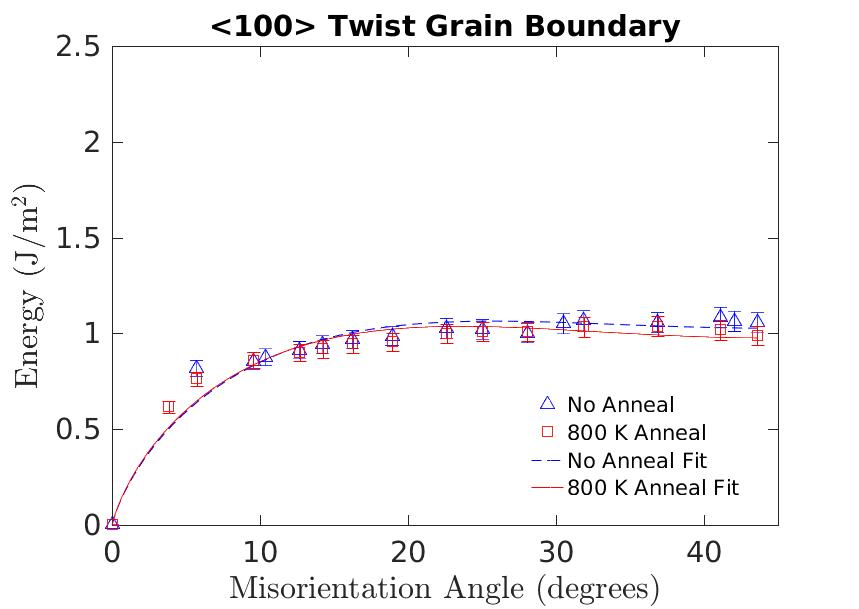
\includegraphics[scale=0.26]{Images/100TwistComparison}}\quad
 \subfloat[]{\label{fig:100Tilt}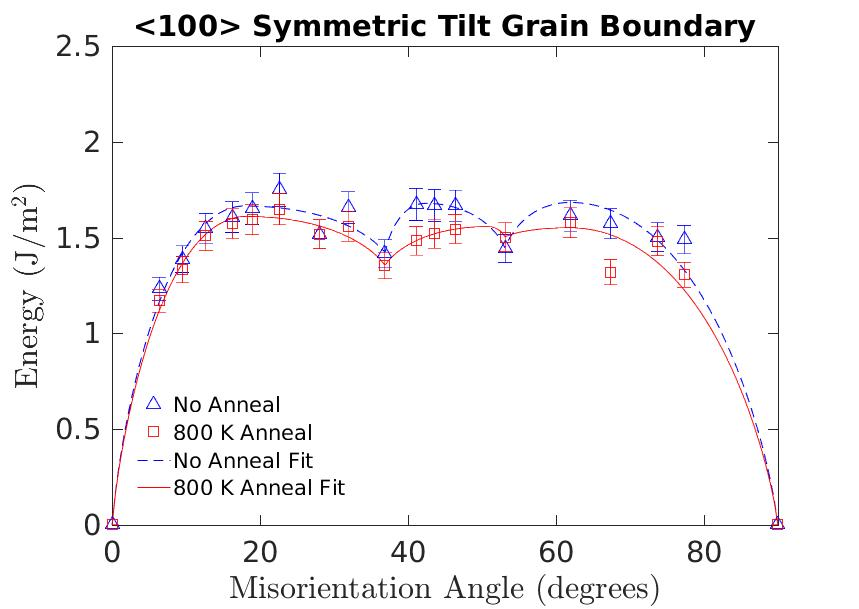
\includegraphics[scale=0.26]{Images/100SymmTiltComparison}}
 \caption[Results for the \textlangle{}100\textrangle{} fitting.]{\label{fig:100} The \textlangle{}100\textrangle{} twist \protect\subref{fig:100Twist} and tilt \protect\subref{fig:100Tilt} results.  In general the re-calculated energies are lower, with significant differences around 40\textdegree{} to 50\textdegree{} in the tilt subset.  The unexpected positive concavity in the twist subset around 40\textdegree{} may indicate the presence of a missing cusp.  Possible cusps exist around 30\textdegree{} in the twist subset, and around 68\textdegree{} in the tilt subset. }
 
\end{figure}

\begin{figure}[ht!]
 \centering
 
 \subfloat[]{\label{fig:110Twist}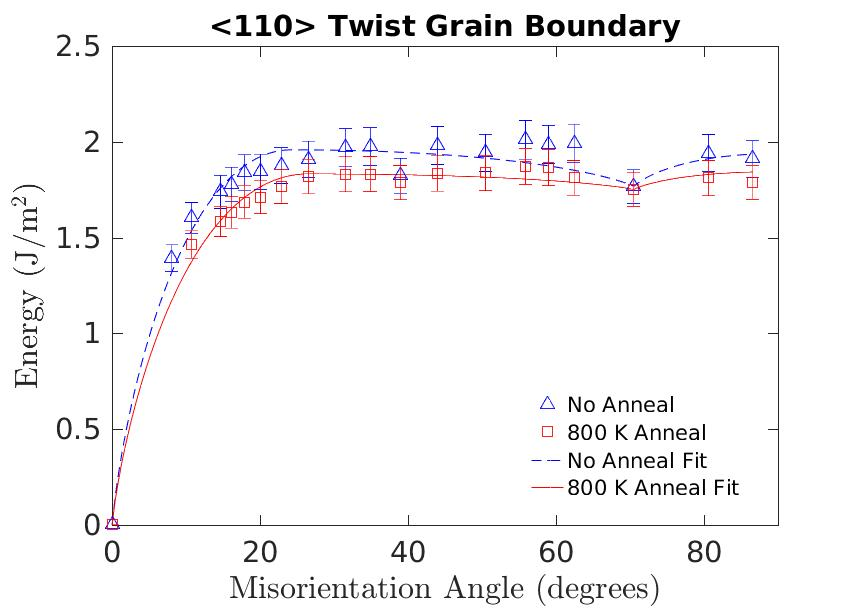
\includegraphics[scale=0.26]{Images/110TwistComparison}}\quad
 \subfloat[]{\label{fig:110Tilt}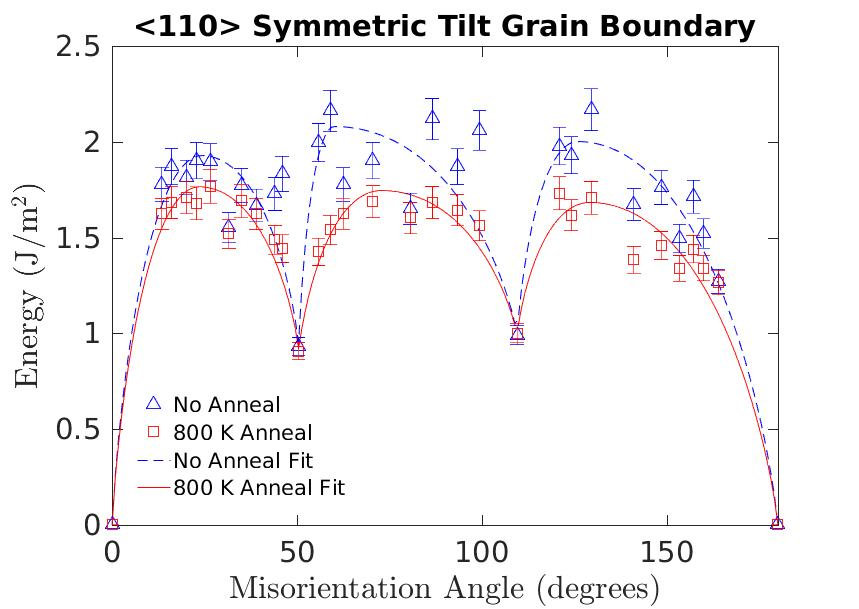
\includegraphics[scale=0.26]{Images/110SymmTiltComparison}}
 \caption[Results for the \textlangle{}110\textrangle{} fitting.]{\label{fig:110} The \textlangle{}110\textrangle{} twist \protect\subref{fig:110Twist} and tilt \protect\subref{fig:110Tilt} results.  Both subsets have significant decreases in energy.  The twist subset has a possible cusp at around 40\textdegree{}, and the tilt subset has possible cusps around 40\textdegree{}, 90\textdegree{}, and 140\textdegree{}.}
 
\end{figure}

\begin{figure}[ht!]
 \centering
 
 \subfloat[]{\label{fig:111Twist}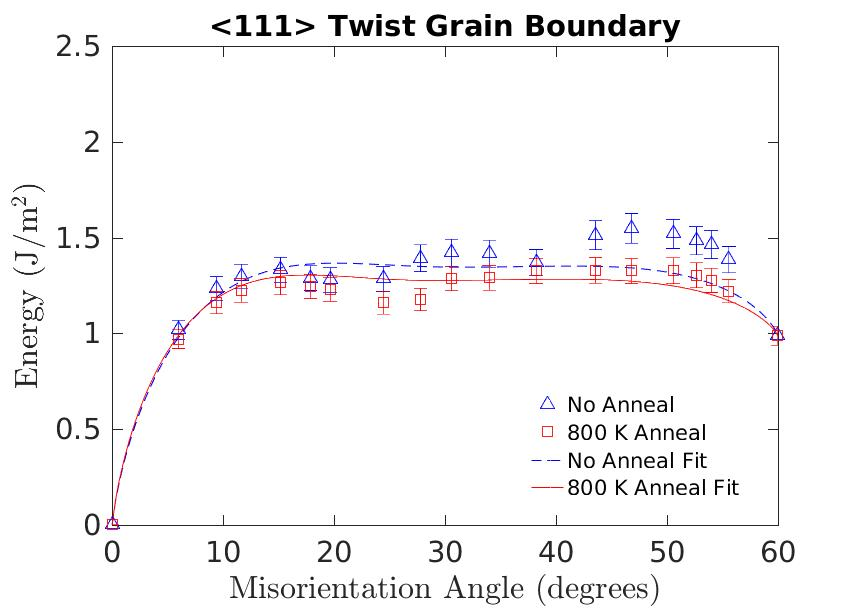
\includegraphics[scale=0.26]{Images/111TwistComparison}}\quad
 \subfloat[]{\label{fig:111Tilt}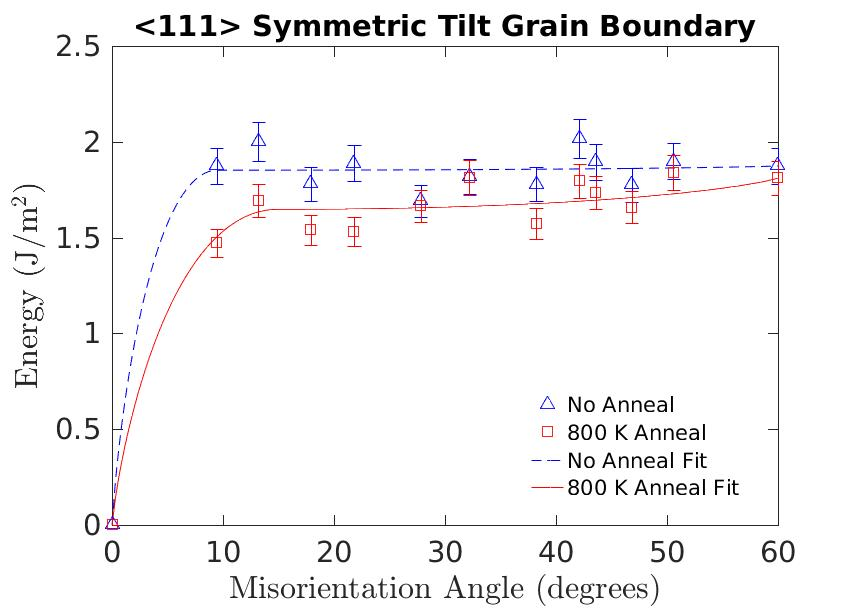
\includegraphics[scale=0.26]{Images/111SymmTiltComparison}}
 \caption[Results for the \textlangle{}111\textrangle{} fitting.]{\label{fig:111} The \textlangle{}111\textrangle{} twist \protect\subref{fig:111Twist} and tilt \protect\subref{fig:111Tilt} results.  Most energies are found to be lower, but some are found to be higher.  The unexpected positive concavity present in these results could indicate the presence of one or more cusps, with one possible location around 33\textdegree{}.  This work needs additional data to determine possible cusp locations for the tilt subset.}
 
\end{figure}

\begin{figure}[ht!]
 \centering
 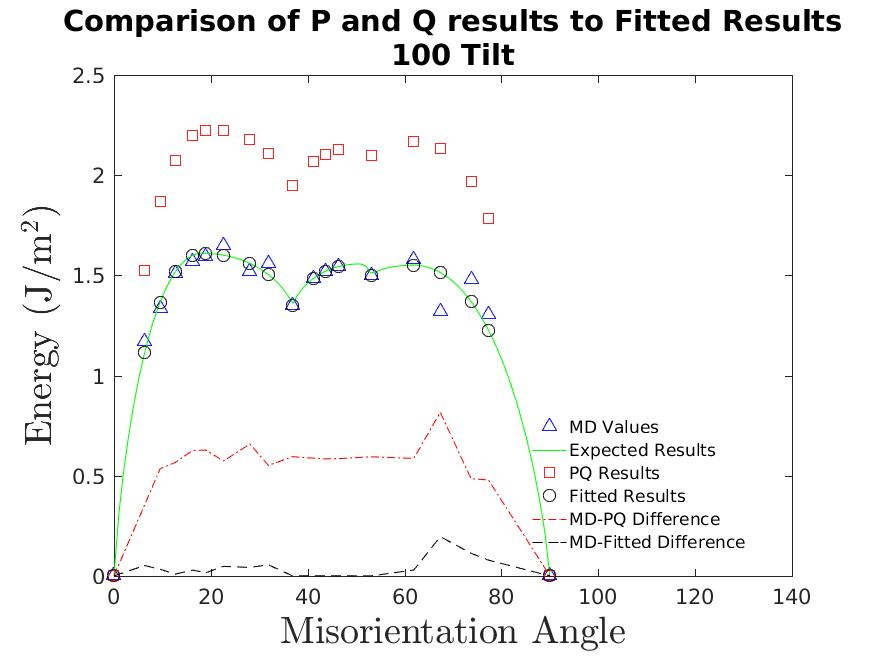
\includegraphics[scale=0.26]{Images/100TiltPQvsMD}
 \caption[Comparison of the PQ matrices with the expected result for \textlangle{}100\textrangle{} tilt.]{\label{fig:100PQ} A comparison of the expected value of the fitted function with the values calculated using the P and Q matrices for the \textlangle{}100\textrangle{} 1D tilt subset, with MD values shown for reference.  The cause of the scaling issue remains unknown.}
\end{figure}

\begin{figure}[ht!]
 
 \begin{minipage}{.5\linewidth}
 \centering
 \subfloat[]{\label{fig:updated100Twist}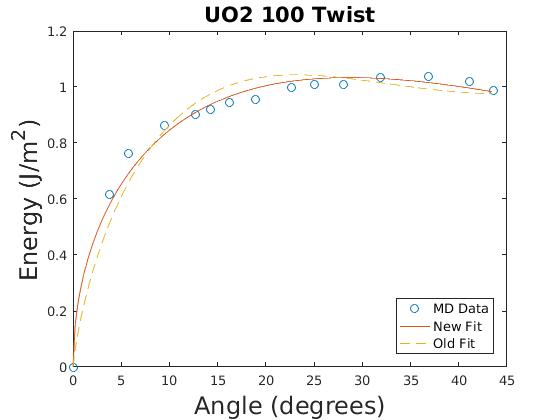
\includegraphics[scale=0.42]{Images/100Twist_marquardt}}
 \end{minipage}%
 \begin{minipage}{.5\linewidth}
 \centering
 \subfloat[]{\label{fig:updated110Twist}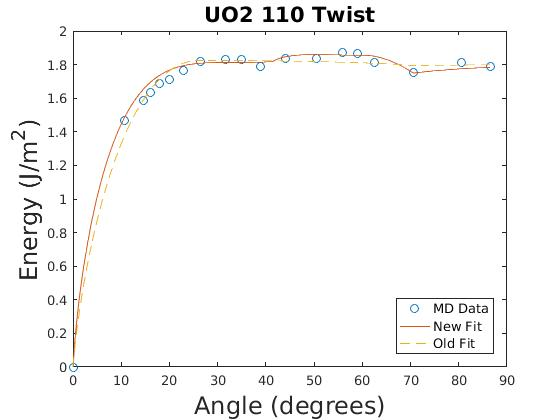
\includegraphics[scale=0.42]{Images/110Twist_vary_shaping_factor}}
 \end{minipage} \par\medskip
 \centering
 \subfloat[]{\label{fig:updated111Twist}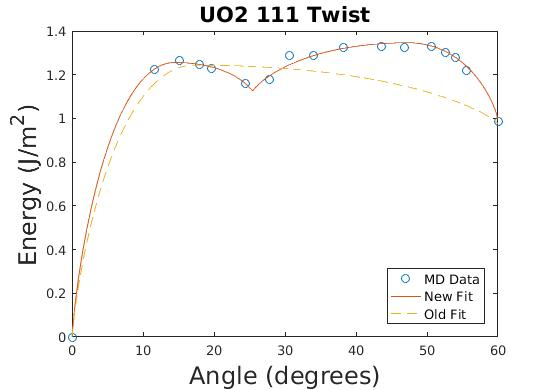
\includegraphics[scale=0.42]{Images/111Twist_marquardt}}
 
 \caption[Possible changes to fitting functions for the 1D twist subsets.]{\label{fig:updatedGraphs} A comparison of current fitting functions with a possible change to the functions.  Dashed lines show the original functions, and the solid lines show the updated functions, with MD results shown for reference. \protect\subref{fig:updated100Twist} shows a possible change from the Read-Shockley-Wolf (RSW) functions to a simple square root function multiplied by an exponential decay without any theoretical basis.  \protect\subref{fig:updated110Twist} attempts to fit to a cusp around 40\textdegree{}.  Further work can be done to find a better fit for this subset. \protect\subref{fig:updated111Twist} shows the most potential improvement.  The potential fit increases the total number of parameters by three to fit to the cusp around 28\textdegree.  A quick glance at the MD values compared to the fit shows a great improvement from the current fit.  To create the graph shown in \protect\subref{fig:updated111Twist} this work spliced two additional RSW functions into the original function.  This created a total of four RSW functions for this subset.}
 
\end{figure}

\section{Reduced Chi-square Results\label{results:chi2red}}
The $\chi_{\textnormal{red}}^2$ values are much smaller than one for every data set regardless of the method used to calculate the statistic, with the exception of the \textlangle{}100\textrangle{} symmetric tilt subset using the P and Q matrices.  This subset has a high $\chi_{\textnormal{red}}^2$ value due to the scaling issue.  Because of the low $\chi_{\textnormal{red}}^2$ values, the fitted functions overfit the data.\cite{bevington2003}  \Cref{table:chi2} lists the $\chi_{\textnormal{red}}^2$ values for the 1D subsets using the two different methods for calculation. 

\begin{table}[ht!]
\centering
\caption{A list of the $\chi_{\textnormal{red}}^2$ results using two different methods: using the P and Q matrices for the various orientations to test the fit, and comparing the results of the 1D fits to the 1D data.  The values for $\chi_{\textnormal{red}}^2$ are all less than one with the exception of the \textlangle{}100\textrangle{} symmetric tilt using the P and Q matrices.  These values indicate an over-fit to the data.}
\label{table:chi2}
\begin{tabular}{{l c c c c}}
1D Subset & \multicolumn{2}{c}{$\chi_{\textnormal{red}}^2$ using P and Q matrices} & \multicolumn{2}{c}{$\chi_{\textnormal{red}}^2$ comparing the 1D fits} \\[5pt]
          & No Anneal & 800 K Anneal & No Anneal & 800 K Anneal \\
\hline
\textlangle{}100\textrangle{} Twist & 0.0953 & 0.1074 & 0.0752 & 0.0722 \\
\textlangle{}110\textrangle{} Twist & 0.1010 & 0.1874 & 0.0400 & 0.0137 \\
\textlangle{}111\textrangle{} Twist & 0.3041 & 0.1139 & 0.4966 & 0.1516 \\
\textlangle{}100\textrangle{} Tilt & 0.1038 & 8.7702 & 0.0846 & 0.0932 \\
\textlangle{}110\textrangle{} Tilt & 4.9799 & 0.3277 & 0.5951 & 0.1762 \\
\textlangle{}111\textrangle{} Tilt & 0.1566 & 0.7814 & 0.1315 & 0.1355 \\
\hline
Overall $\chi_{\textnormal{red}}^2$ & 1.7652 & 1.4893 & 0.2678 & 0.1153 \\
\end{tabular}
\end{table}

\chapter{Conclusion\label{conclusion}}
This work has successfully created a more accurate interpolation function for grain boundary (GB) energies in uranium dioxide (UO\textsubscript{2}), but revealed additional characteristics of the full five-dimensional (5D) GB space that require further research.  GB energies were found to be lower when calculated with an 800 K anneal as expected when compared to the data set created without an anneal.  Descriptions of those additional characteristics through the use of additional functions will prove beneficial.  

Future work should focus on calculating additional data points for fitting.  Increasing the number of data points will improve the quality of the fit.  Additional data points will also help to identify trends that do not readily appear with the limited data currently available. 

Further work could generalize this function to all polycrystalline materials with the fluorite crystal structure.  Such a generalization would provide further validation of this model, however, such validation would require a sufficient number of GB energies for many different materials with such a structure.  The literature does not provide these energies, indicating a need for additional computational resources.

As the model develops, initial conditions set by actual nuclear fuel data will be put into a MARMOT simulation.  After simulating grain growth in a nuclear reactor, the fuel data will be compared with the simulation data to determine the accuracy of the model.

% Start labeling chapters with letters and calling them appendices
\appendix
\renewcommand\chaptername{Appendix}

 % Make the bibliography.
 \cleardoublepage
 \bibliography{gbCharacter}

\chapter{List of Parameters\label{app:params}}

\begin{longtable}{r l l}
\label{table:params}\\
\caption{This table gives the parameters for UO\textsubscript{2} that generate the energy profiles.}\\
\hline
\hline
Array number & Parameter name & Parameter value \\
\hline
\endfirsthead
\multicolumn{3}{c}{\tablename\ \thetable\ -- \textit{Continued from previous page}}\\
\hline
Array number & Parameter name & Parameter value \\
\hline
\endhead
\hline
\multicolumn{3}{r}{\textit{Continued on next page.}}\\
\endfoot
\hline
\hline
\endlastfoot
1 & Energy Scaling Factor ($e_{RGB}$) & 1.6012 $J/m^2$ \\
2 & \textlangle{}100\textrangle{} Max Distance & 0.405 \\
3 & \textlangle{}110\textrangle{} Max Distance & 0.739 \\
4 & \textlangle{}111\textrangle{} Max Distance & 0.352 \\
5 & \textlangle{}100\textrangle{} Weight & 85.3 \\
6 & \textlangle{}110\textrangle{} Weight & 6.95 \\
7 & \textlangle{}111\textrangle{} Weight & 0.08 \\
8 & \textlangle{}100\textrangle{} Tilt/Twist Mix Power Law (1) & 0.03325 \\
9 & \textlangle{}100\textrangle{} Tilt/Twist Mix Power Law (2) & 0.00053125 \\
10 & Maximum \textlangle{}100\textrangle{} Twist Energy & 0.60903 \\
11 & \textlangle{}100\textrangle{} Twist Shape Factor & 1.4486 \\
12 & \textlangle{}100\textrangle{} Asymmetric Tilt Interpolation Power & 36.2 \\
13 & \textlangle{}100\textrangle{} Symmetric Tilt First Peak Energy & 1.0058 \\
14 & \textlangle{}100\textrangle{} Symmetric Tilt First $\Sigma5$ Energy & 0.84456 \\
15 & \textlangle{}100\textrangle{} Symmetric Tilt Second Peak Energy & 0.97259 \\
16 & \textlangle{}100\textrangle{} Symmetric Tilt Second $\Sigma5$ Energy & 0.9379 \\
17 & \textlangle{}100\textrangle{} Symmetric Tilt $\Sigma17$ Energy & 0.96881 \\
18 & \textlangle{}100\textrangle{} Symmetric Tilt First Peak Angle & 0.31569 \\
19 & \textlangle{}100\textrangle{} Symmetric Tilt Second Peak Angle & 0.88538 \\
20 & \textlangle{}110\textrangle{} Tilt/Twist Mix Power Law (1) & 10.257 \\
21 & \textlangle{}110\textrangle{} Tilt/Twist Mix Power Law (2) & 3.5784 \\
22 & \textlangle{}110\textrangle{} Twist Peak Angle & 0.46145 \\
23 & \textlangle{}110\textrangle{} Twist Peak Energy & 1.1444 \\
24 & \textlangle{}110\textrangle{} Twist $\Sigma3$ Energy & 1.0931 \\
25 & \textlangle{}110\textrangle{} Twist 90\textdegree{} Energy & 1.152 \\
26 & \textlangle{}110\textrangle{} Asymmetric Tilt Shape Factor & 3.1843 \\
27 & \textlangle{}110\textrangle{} Symmetric Tilt Third Peak Energy & 1.0514 \\
28 & \textlangle{}110\textrangle{} Symmetric Tilt $\Sigma3$ Energy & 0.61703 \\
29 & \textlangle{}110\textrangle{} Symmetric Tilt Second Peak Energy & 1.0902 \\
30 & \textlangle{}110\textrangle{} Symmetric Tilt $\Sigma11$ Energy & 0.56686 \\
31 & \textlangle{}110\textrangle{} Symmetric Tilt First Peak Energy & 1.1024 \\
32 & \textlangle{}110\textrangle{} Symmetric Tilt Third Peak Angle & 0.88736 \\
33 & \textlangle{}110\textrangle{} Symmetric Tilt Second Peak Angle & 1.8711 \\
34 & \textlangle{}110\textrangle{} Symmetric Tilt First Peak Angle & 2.731 \\
35 & \textlangle{}111\textrangle{} Tilt-Twist Linear Interpolation & 66.101 \\
36 & \textlangle{}111\textrangle{} Twist Shape Factor & 1.2414 \\
37 & \textlangle{}111\textrangle{} Twist Peak Angle & 0.49979 \\
38 & \textlangle{}111\textrangle{} Twist Peak Energy & 0.7971 \\
39 & \textlangle{}111\textrangle{} Symmetric Tilt Peak Angle & 0.25966 \\
40 & \textlangle{}111\textrangle{} Symmetric Tilt Max Energy & 1.0288 \\
41 & \textlangle{}111\textrangle{} Symmetric Tilt $\Sigma3$ Energy & 1.1311 \\
42 & \textlangle{}111\textrangle{} Asymmetric Tilt Symmetry Point Energy & 3.3314 \\
43 & \textlangle{}111\textrangle{} Asymmetric Tilt Scale Factor & 0.065136 \\
\end{longtable}

\chapter{Grain Boundary Representations\label{app:gbRep}}
Visual representations of the GB space helped Bulatov \emph{et al.} develop their 5D function.  However, the size of the five-space in which GBs reside makes representing them difficult.  Researchers have developed different methods to represent them, each with their advantages and disadvantages.  Three of these methods are the axis-angle representation, the Rodrigues representation, and the fundamental zone representation.  These methods, though described separately, can be used together to form a better picture of what the GB space looks like (see for example \Cref{fig:bulatovRodrigues} which combines the Rodrigues representation and the fundamental zone representation).

\section{Axis-Angle Representation\label{GBReps:AA}}
Of the three described, the axis-angle representation most simplistically describes GB space.  The axis of rotation of the GB specifies the point in axis-angle space, and the angle of misorientation between the two grains at the GB specifies the magnitude of the vector.  Thus, the axis ($\bm{a}$) and the angle ($\theta$) mathematically represent an axis-angle vector as:
\begin{equation}
\bm{A} = \bm{a}\ \theta
\label{eq:aaVec}
\end{equation} 

The axis-angle space can only take into account three degrees of freedom: the two angles specifying the axis, and the angle rotated through.  Thus, axis-angle space cannot fully visualize all of the necessary information contained in the full 5D space.\cite{frank1988} This representation suffers from the difficulties of understanding an infinite space because it maps an axis and an angle onto a Cartesian coordinate system.  Without the help of additional methods, this infinite space remains difficult to understand.  The best uses of this representation focus on using it as a starting point to move to other, more robust representations, and to represent the misorientation between two grains.\cite{randle2000}

\section{Rodrigues Representation\label{GBReps:Rodrigues}}
The Rodrigues representation (sometimes called the ``Rodrigues-Frank" representation) uses Rodrigues vectors to represent rotations in Rodrigues space.  This representation takes ideas from the axis-angle space, but makes a few changes allowing crystal symmetries to be taken into account.  The orientation of the GB normal still specifies the point in space, but the tangent of half the angle represents the magnitude of the vector. Thus, a Rodrigues vector can be represented as:\cite{morawiec1996, becker1989, frank1988, randle2000, priester2013}
\begin{equation}
\bm{R}=\bm{a}\ \textnormal{tan}\left(\frac{\theta}{2}\right)
\label{eq:rodriguesVec}
\end{equation}
Some researchers favor this representation over others because of the lack of curvature such a mapping entails.\cite{frank1988, randle2000}  However, it still only specifies three of the five degrees of freedom.  Bulatov \emph{et al.}\ attached a unit vector at the points along the axis to represent the other two DoFs in \Cref{fig:bulatovRodrigues}. A parallel vector represents a twist boundary, and a perpendicular vector represents a tilt boundary.  Anything else represents a mix of twist and tilt (or a mixed boundary).  One limitation of Rodrigues space lies in that it also maps to an infinite space.\cite{frank1988, kirch2008}.

\section{Fundamental Zone Representation\label{GBReps:FunZone}}
The fundamental zone graphically represents the full 5D GB best.  This representation takes advantage of the symmetries inherent in crystals\cite{stokes2007} to simplify an infinite space into a compact, finite area called the fundamental zone.\cite{bulatov2014, patala2013, homer2015, morawiec1996, patala2012}  Every point within the space represents a unique orientation, and every point outside the space can be represented as a point inside the space through symmetry operations.\cite{morawiec1996, becker1989, frank1988}  Bulatov \emph{et al.}\ used this idea in connection with Rodrigues space to create \Cref{fig:bulatovRodrigues}.  In Rodrigues space, the crystal symmetries of the material determine the shape of the fundamental zone.\cite{patala2013, morawiec1996}  For fcc crystals, the fundamental zone takes the form of a truncated tetrahedron.\cite{bulatov2014}  The edges of the fundamental zone in Rodrigues space represent the high-symmetry rotation axes, and points on one face can represent another point on a different face of the fundamental zone.  

\chapter{Graphs\label{app:graphs}}
\begin{figure}[ht!]
 \centering
 
 \subfloat[]{\label{appfig:compare100Twist}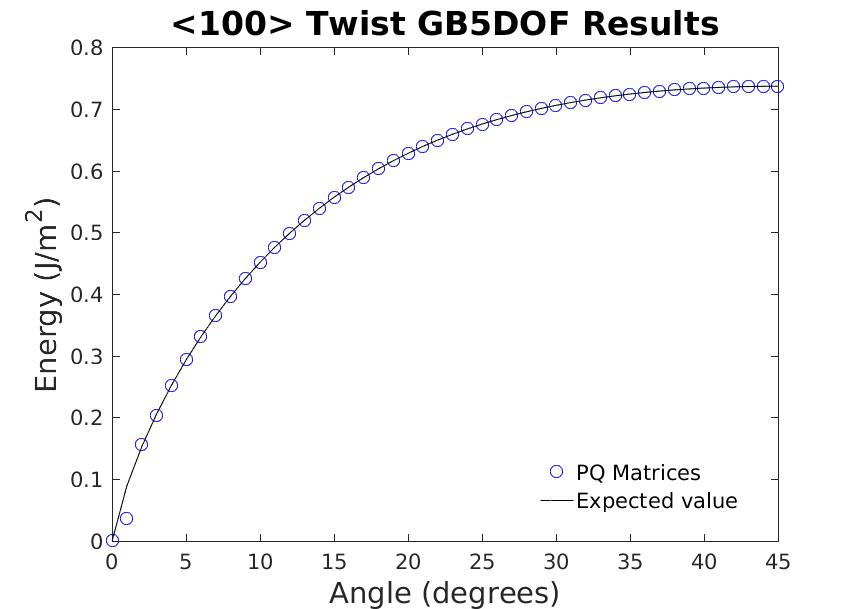
\includegraphics[scale=0.24]{Images/TestPQFit100Twist}}\quad
 \subfloat[]{\label{appfig:compare100Tilt}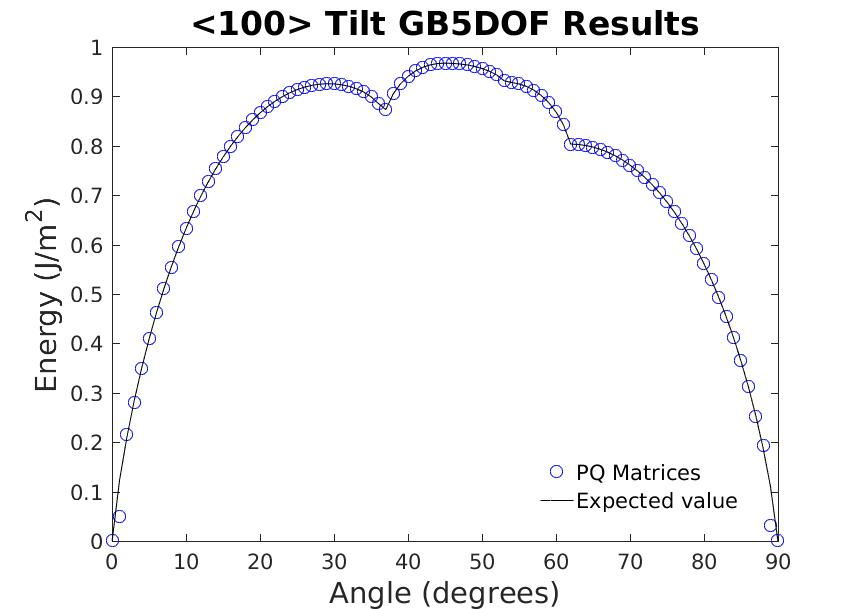
\includegraphics[scale=0.26]{Images/TestPQFit100Tilt}}
 \caption[A comparison of the \textlangle{}100\textrangle{} copper curves with the calculated results.]{\label{appfig:compare100} The \textlangle{}100\textrangle{} twist \protect\subref{appfig:compare100Twist} and tilt \protect\subref{appfig:compare100Tilt} results for the P and Q matrices as compared to Bulatov \emph{et al.}'s energy profiles. Bulatov \emph{et al.}'s \lstinline!GB5DOF.m! MATLAB\textsuperscript{\textregistered} script calculated the expected values by using the default parameters.  The \lstinline!GB5DOF.m! script calculated the values using the generated matrices.  With the exception of the data points at 1\textdegree{} in both \protect\subref{appfig:compare100Twist} and \protect\subref{appfig:compare100Tilt} and 89\textdegree{} in \protect\subref{appfig:compare100Tilt}, the energies calculated from the matrices matches the expected curves exactly.}
\end{figure}

\begin{figure}[ht!]
 \centering
 
 \subfloat[]{\label{appfig:compare110Twist}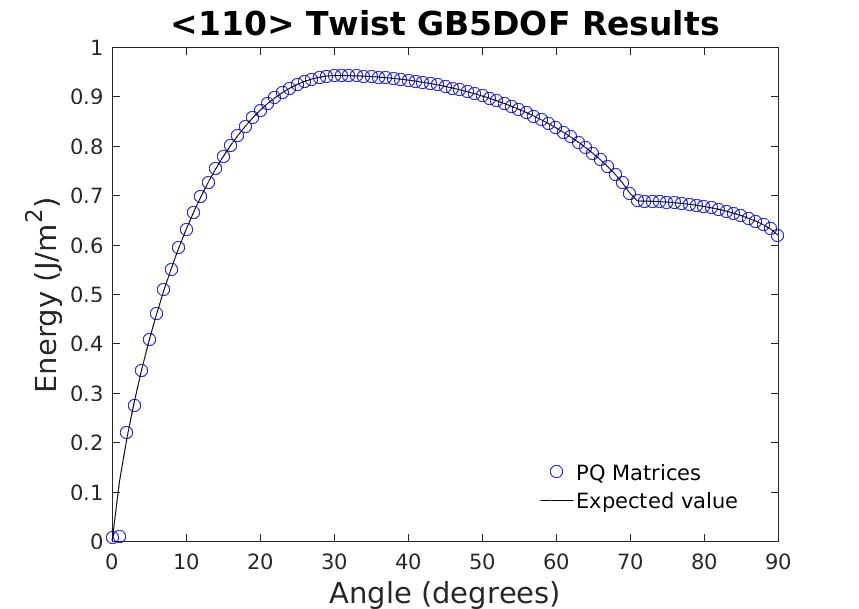
\includegraphics[scale=0.24]{Images/TestPQFit110Twist}}\quad
 \subfloat[]{\label{appfig:compare110Tilt}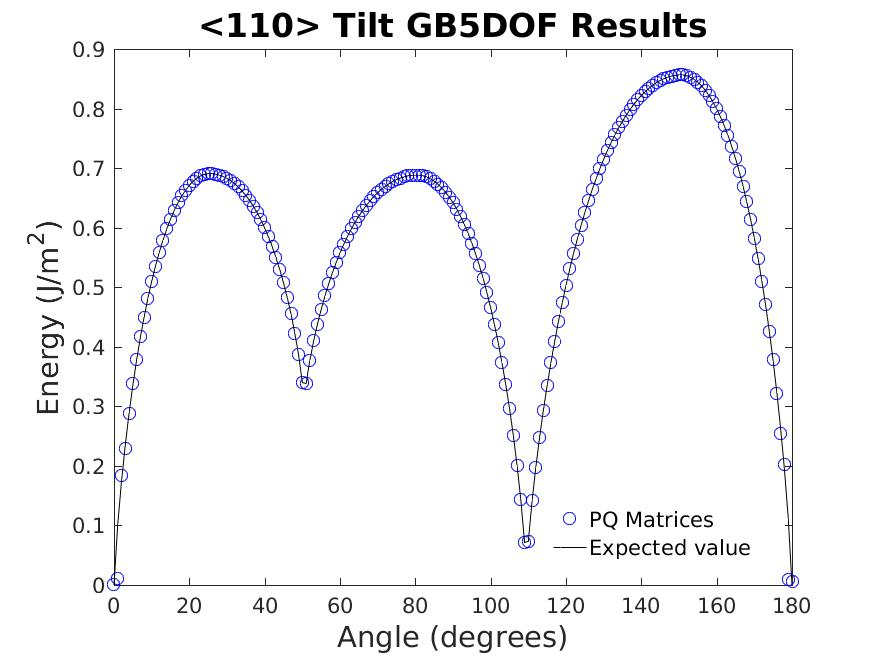
\includegraphics[scale=0.26]{Images/TestPQFit110Tilt}}
 \caption[A comparison of the \textlangle{}110\textrangle{} copper curves with the calculated results.]{\label{appfig:compare110} The \textlangle{}110\textrangle{} twist \protect\subref{appfig:compare110Twist} and tilt \protect\subref{appfig:compare110Tilt} results for the P and Q matrices as compared to Bulatov \emph{et al.}'s energy profiles. Bulatov \emph{et al.}'s \lstinline!GB5DOF.m! MATLAB\textsuperscript{\textregistered} script calculated the expected values by using the default parameters.  The \lstinline!GB5DOF.m! script calculated the values using the generated matrices. With the exception of the data points at 1\textdegree{} in both \protect\subref{appfig:compare110Twist} and \protect\subref{appfig:compare110Tilt} and 179\textdegree{} in \protect\subref{appfig:compare110Tilt}, the energies calculated from the matrices matches the expected curves exactly.}
\end{figure}

\begin{figure}[ht!]
 \centering
 
 \subfloat[]{\label{appfig:compare111Twist}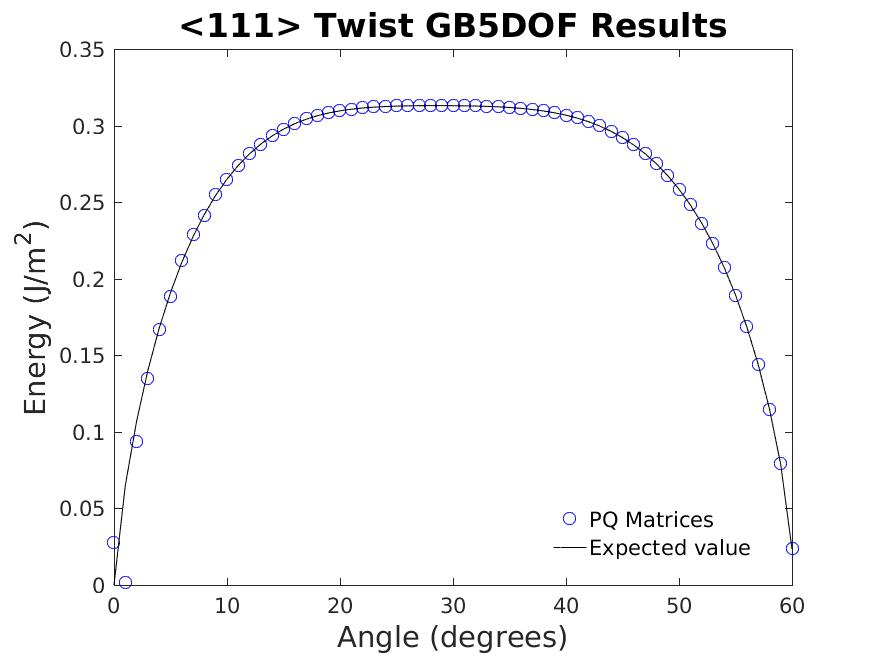
\includegraphics[scale=0.24]{Images/TestPQFit111Twist}}\quad
 \subfloat[]{\label{appfig:compare111Tilt}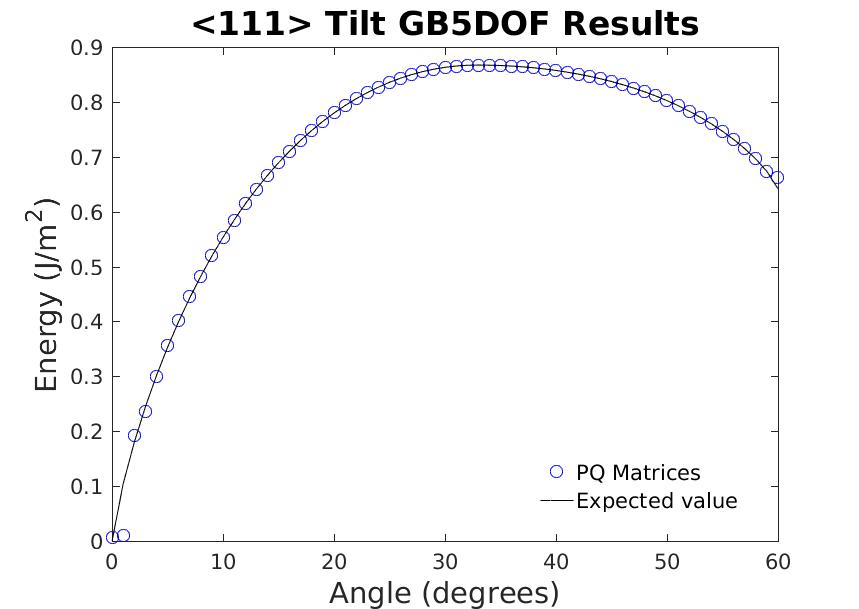
\includegraphics[scale=0.26]{Images/TestPQFit111Tilt}}
 \caption[A comparison of the \textlangle{}111\textrangle{} copper curves with the calculated results.]{\label{appfig:compare111} The \textlangle{}111\textrangle{} twist \protect\subref{appfig:compare111Twist} and tilt \protect\subref{appfig:compare111Tilt} results for the P and Q matrices as compared to Bulatov \emph{et al.}'s energy profiles. Bulatov \emph{et al.}'s \lstinline!GB5DOF.m! MATLAB\textsuperscript{\textregistered} script calculated the expected values by using the default parameters. The \lstinline!GB5DOF.m! script calculated the values using the generated matrices. With the exception of the data points at 1\textdegree{} in both \protect\subref{appfig:compare111Twist} and \protect\subref{appfig:compare111Tilt} and 60\textdegree{} in \protect\subref{appfig:compare111Tilt}, the energies calculated from the matrices matches the expected curves exactly.}
\end{figure}

\begin{figure}[ht!]
 \centering
 
 \subfloat[]{\label{appfig:100TwistPQ}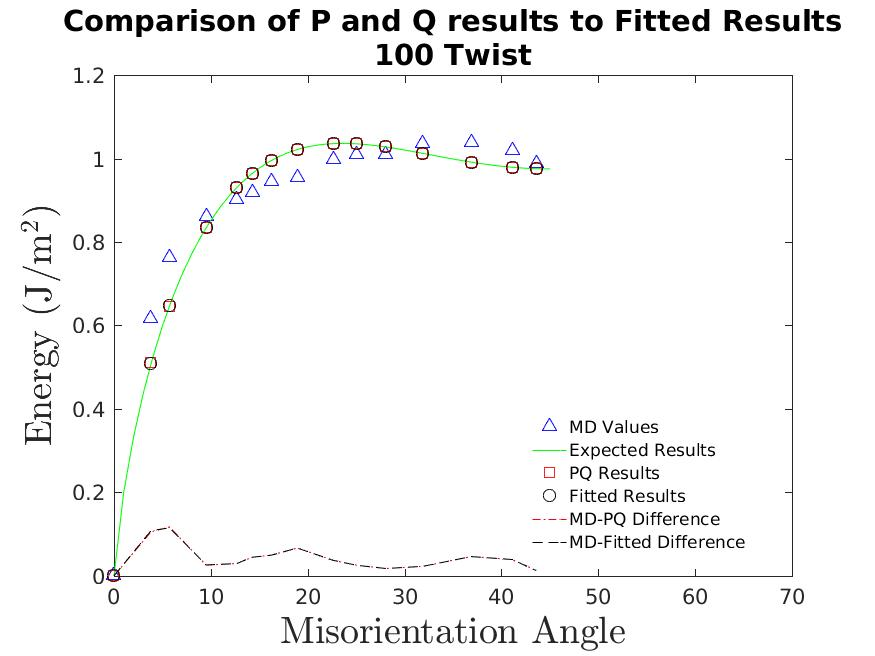
\includegraphics[scale=0.26]{Images/100TwistPQvsMD}}\quad
 \subfloat[]{\label{appfig:100TiltPQ}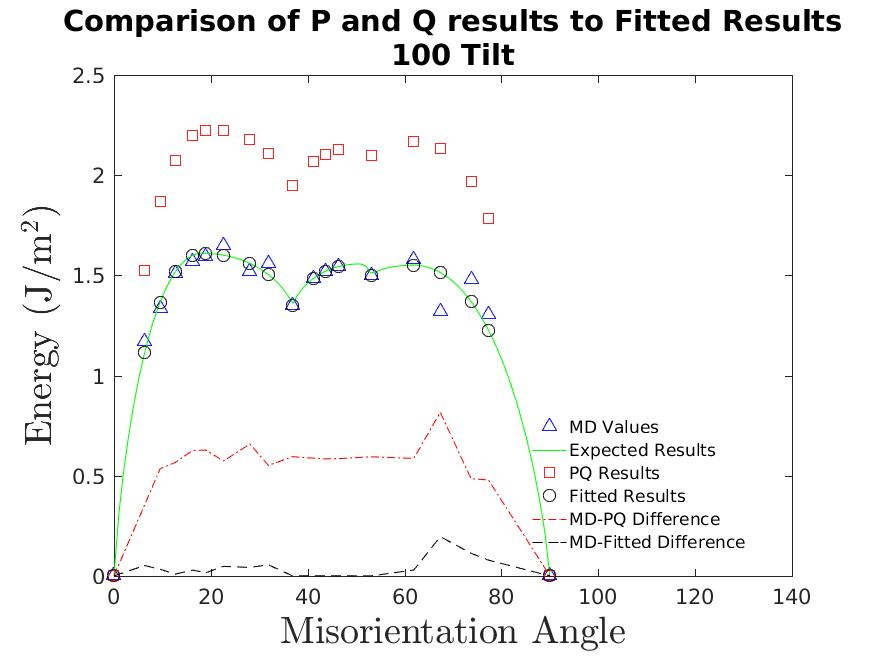
\includegraphics[scale=0.26]{Images/100TiltPQvsMD}}
 \caption[Comparison of the PQ matrices with the expected result for \textlangle{}100\textrangle{} 1D subset.]{\label{appfig:100PQ} A comparison of the expected value of the fitted function with the values calculated using the P and Q matrices for the \textlangle{}100\textrangle{} 1D subsets, with the MD values shown for reference.  \protect\subref{appfig:100TwistPQ} PQ results follow exactly the fitted curve.  \protect\subref{appfig:100TiltPQ} has a scaling issue yet to be fixed.  The cause of the scaling issue remains unknown.}
\end{figure}

\begin{figure}[ht!]
 \centering
 
 \subfloat[]{\label{appfig:110TwistPQ}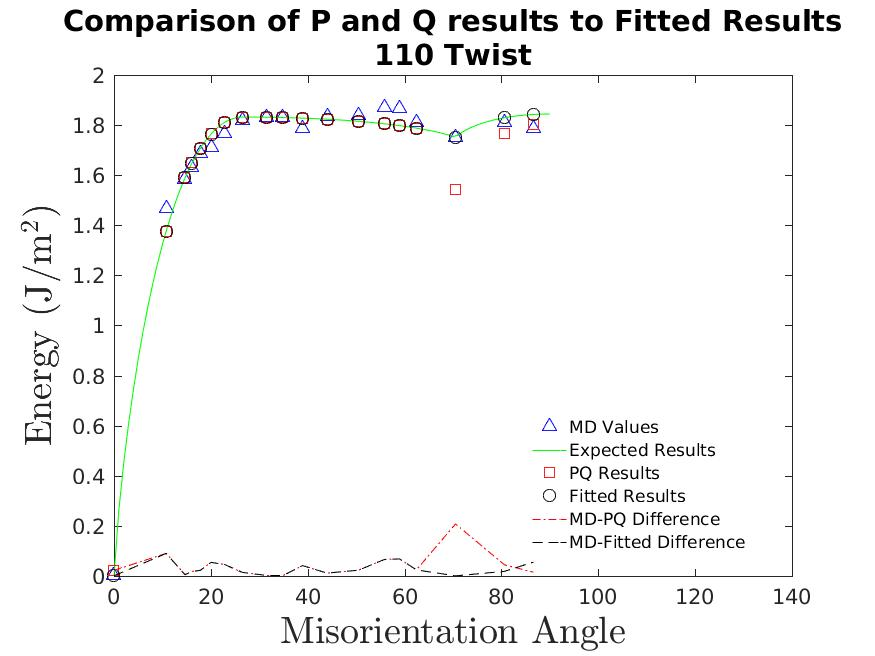
\includegraphics[scale=0.26]{Images/110TwistPQvsMD}}\quad
 \subfloat[]{\label{appfig:110TiltPQ}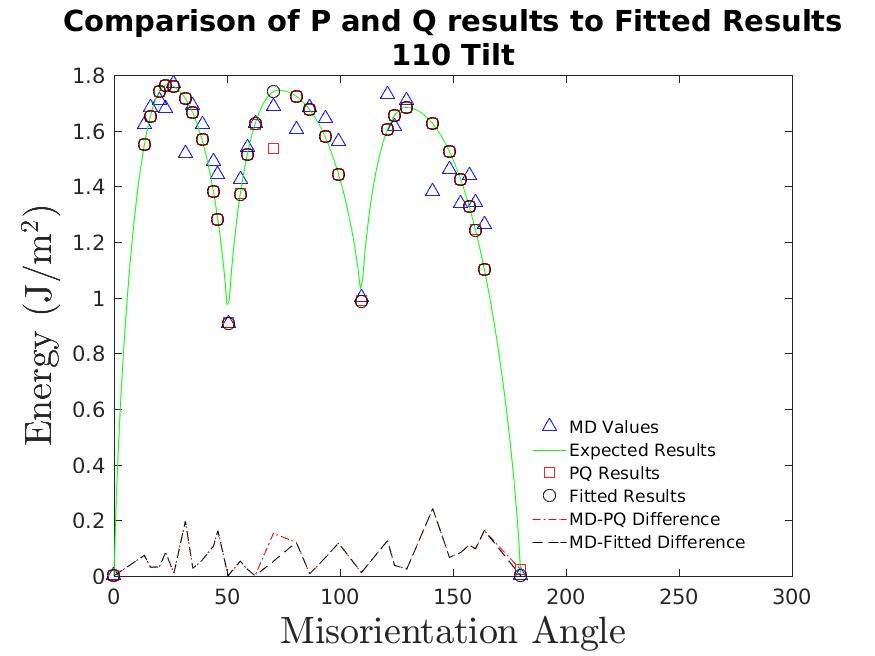
\includegraphics[scale=0.26]{Images/110TiltPQvsMD}}
 \caption[Comparison of the PQ matrices with the expected result for \textlangle{}110\textrangle{} 1D subset.]{\label{appfig:110PQ} A comparison of the expected value of the fitted function with the values calculated using the P and Q matrices for the \textlangle{}110\textrangle{} 1D subsets, with the MD values shown for reference.  \protect\subref{appfig:110TwistPQ} follows the fitted result until the cusp, at which point some anomalies appear.  The results from the PQ matrices dip well below the expected value at the cusp, and never make it back to the original fitted line. \protect\subref{appfig:110TiltPQ} has a similar issue on a lesser scale.  Only two of the calculated points do not follow the fitted curve.  At the endpoint the expected value is zero, but the PQ matrices calculated a value slightly higher.  Also, an unexpected cusp from the PQ matrices appears in the middle of the second hump.  All other data points follow the fitted curve exactly.}
\end{figure}

\begin{figure}[ht!]
 \centering
 
 \subfloat[]{\label{appfig:111TwistPQ}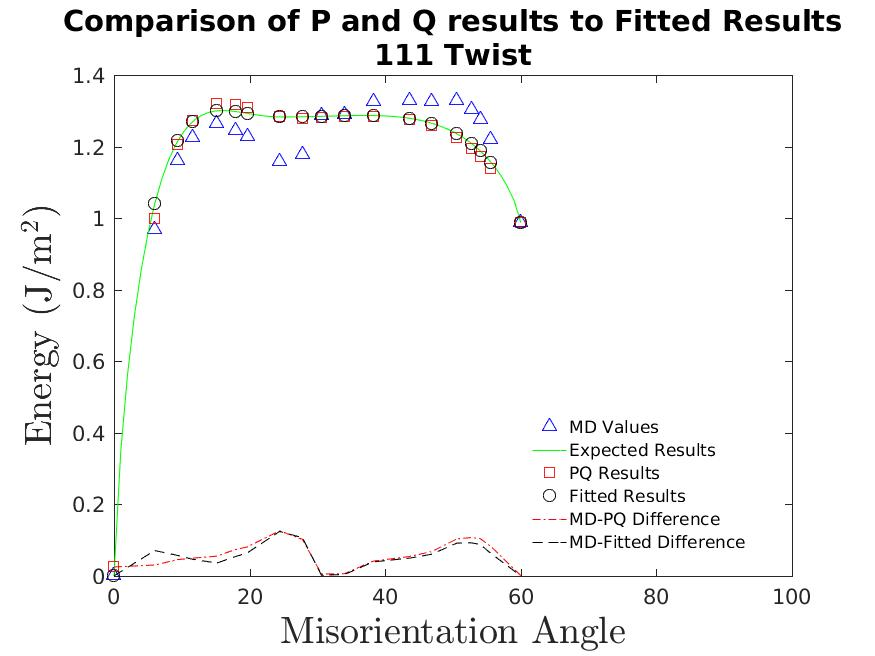
\includegraphics[scale=0.26]{Images/111TwistPQvsMD}}\quad
 \subfloat[]{\label{appfig:111TiltPQ}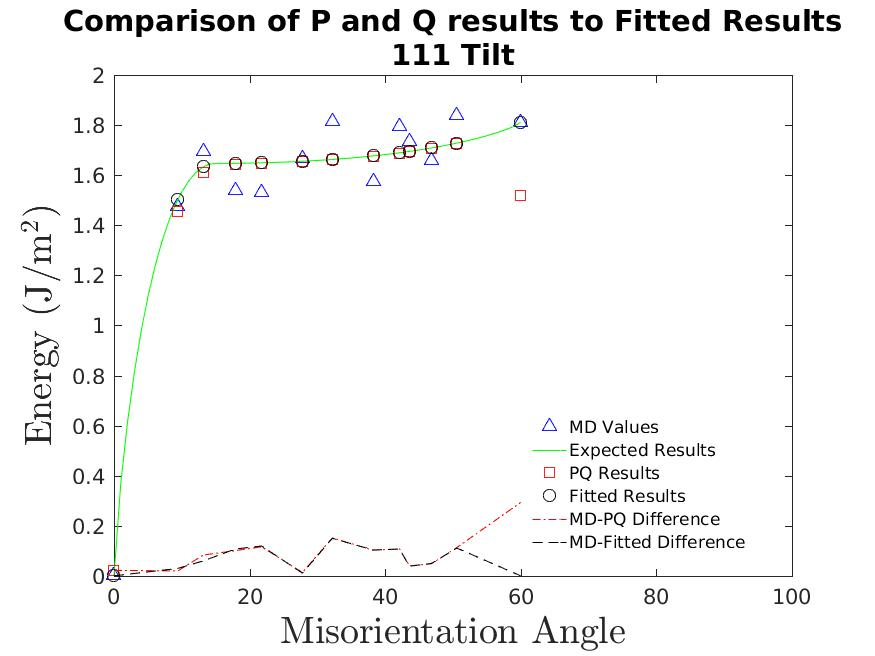
\includegraphics[scale=0.26]{Images/111TiltPQvsMD}}
 \caption[Comparison of the PQ matrices with the expected result for \textlangle{}111\textrangle{} 1D subset.]{\label{appfig:111PQ} A comparison of the expected value of the fitted function with the values calculated using the P and Q matrices for the \textlangle{}111\textrangle{} 1D subsets, with the MD values shown for reference.  \protect\subref{appfig:111TwistPQ} closely follows the expected fitted values, but has a slight error throughout.  \protect\subref{appfig:111TiltPQ} follows the expected values exactly in the center of the fitting, but misses slightly for lower angle boundaries, and misses completely at the end.}
\end{figure}

\chapter{Orientation Matrix Generator\label{app:OrientationMatrix}}
This code generates the orientation matrices (known as the P and Q matrices in Bulatov \emph{et al.}'s code). Provision for calculating the matrices one of two ways appears in-code through the use of command-line options.

\lstinputlisting[language=Python, breaklines=true, firstline=61]{../../scripts/orientation_matrix.py}

\chapter{Rotation Matrix Generator\label{app:RotationMatrix}}
This code generates the rotation matrices used to rotate the axes to the [100] direction as required by Bulatov \emph{et al.}'s script.

\lstinputlisting[language=Python, breaklines=true, firstline=25]{../../scripts/rotation_matrix.py}

\chapter{genOrientationMatrix.sh Bash Script\label{app:genOrientationMatrix}}
This bash script reads a CSV file containing misorientation angles data, and uses those angles to generate the P and Q matrices.  This script calls the script \lstinline!orientation_matrix.py!.

\lstinputlisting[language=Bash,breaklines=true]{../../scripts/genOrientationMatrices.sh}
%%%%%%%%%%%%%%%%%%%%%%%%%%%%%%%%%%%%%%%%%%%%%%%%%%%%%%%%%%%%%%%%%%%%%%%%%%%%%


 % Make the index
 \cleardoublepage
 \singlespace
 % NOTE: '\phantomsection' helps get the pdf bookmark to work right. You need
 % to put it before every manual addition to the table of contents
 \phantomsection
 \addcontentsline{toc}{chapter}{Index}
 \printindex

\end{document}
